% Options for packages loaded elsewhere
\PassOptionsToPackage{unicode}{hyperref}
\PassOptionsToPackage{hyphens}{url}
%
\documentclass[
  11pt,
]{article}
\usepackage{amsmath,amssymb}
\usepackage{lmodern}
\usepackage{iftex}
\ifPDFTeX
  \usepackage[T1]{fontenc}
  \usepackage[utf8]{inputenc}
  \usepackage{textcomp} % provide euro and other symbols
\else % if luatex or xetex
  \usepackage{unicode-math}
  \defaultfontfeatures{Scale=MatchLowercase}
  \defaultfontfeatures[\rmfamily]{Ligatures=TeX,Scale=1}
\fi
% Use upquote if available, for straight quotes in verbatim environments
\IfFileExists{upquote.sty}{\usepackage{upquote}}{}
\IfFileExists{microtype.sty}{% use microtype if available
  \usepackage[]{microtype}
  \UseMicrotypeSet[protrusion]{basicmath} % disable protrusion for tt fonts
}{}
\makeatletter
\@ifundefined{KOMAClassName}{% if non-KOMA class
  \IfFileExists{parskip.sty}{%
    \usepackage{parskip}
  }{% else
    \setlength{\parindent}{0pt}
    \setlength{\parskip}{6pt plus 2pt minus 1pt}}
}{% if KOMA class
  \KOMAoptions{parskip=half}}
\makeatother
\usepackage{xcolor}
\IfFileExists{xurl.sty}{\usepackage{xurl}}{} % add URL line breaks if available
\IfFileExists{bookmark.sty}{\usepackage{bookmark}}{\usepackage{hyperref}}
\hypersetup{
  pdftitle={R\&D Investment and Economic Growth in Europe: A Multi-Method Panel Analysis},
  pdfauthor={Andrei Manoloiu},
  hidelinks,
  pdfcreator={LaTeX via pandoc}}
\urlstyle{same} % disable monospaced font for URLs
\usepackage[margin=2.5cm]{geometry}
\usepackage{longtable,booktabs,array}
\usepackage{calc} % for calculating minipage widths
% Correct order of tables after \paragraph or \subparagraph
\usepackage{etoolbox}
\makeatletter
\patchcmd\longtable{\par}{\if@noskipsec\mbox{}\fi\par}{}{}
\makeatother
% Allow footnotes in longtable head/foot
\IfFileExists{footnotehyper.sty}{\usepackage{footnotehyper}}{\usepackage{footnote}}
\makesavenoteenv{longtable}
\usepackage{graphicx}
\makeatletter
\def\maxwidth{\ifdim\Gin@nat@width>\linewidth\linewidth\else\Gin@nat@width\fi}
\def\maxheight{\ifdim\Gin@nat@height>\textheight\textheight\else\Gin@nat@height\fi}
\makeatother
% Scale images if necessary, so that they will not overflow the page
% margins by default, and it is still possible to overwrite the defaults
% using explicit options in \includegraphics[width, height, ...]{}
\setkeys{Gin}{width=\maxwidth,height=\maxheight,keepaspectratio}
% Set default figure placement to htbp
\makeatletter
\def\fps@figure{htbp}
\makeatother
\setlength{\emergencystretch}{3em} % prevent overfull lines
\providecommand{\tightlist}{%
  \setlength{\itemsep}{0pt}\setlength{\parskip}{0pt}}
\setcounter{secnumdepth}{5}
\usepackage{booktabs}
\usepackage{longtable}
\usepackage{array}
\usepackage{multirow}
\usepackage{wrapfig}
\usepackage{float}
\usepackage{colortbl}
\usepackage{pdflscape}
\usepackage{tabu}
\usepackage{threeparttable}
\usepackage{threeparttablex}
\usepackage[normalem]{ulem}
\usepackage{makecell}
\usepackage{xcolor}
\ifLuaTeX
  \usepackage{selnolig}  % disable illegal ligatures
\fi
\newlength{\cslhangindent}
\setlength{\cslhangindent}{1.5em}
\newlength{\csllabelwidth}
\setlength{\csllabelwidth}{3em}
\newenvironment{CSLReferences}[2] % #1 hanging-ident, #2 entry spacing
 {% don't indent paragraphs
  \setlength{\parindent}{0pt}
  % turn on hanging indent if param 1 is 1
  \ifodd #1 \everypar{\setlength{\hangindent}{\cslhangindent}}\ignorespaces\fi
  % set entry spacing
  \ifnum #2 > 0
  \setlength{\parskip}{#2\baselineskip}
  \fi
 }%
 {}
\usepackage{calc}
\newcommand{\CSLBlock}[1]{#1\hfill\break}
\newcommand{\CSLLeftMargin}[1]{\parbox[t]{\csllabelwidth}{#1}}
\newcommand{\CSLRightInline}[1]{\parbox[t]{\linewidth - \csllabelwidth}{#1}\break}
\newcommand{\CSLIndent}[1]{\hspace{\cslhangindent}#1}

\title{R\&D Investment and Economic Growth in Europe: A Multi-Method Panel Analysis}
\usepackage{etoolbox}
\makeatletter
\providecommand{\subtitle}[1]{% add subtitle to \maketitle
  \apptocmd{\@title}{\par {\large #1 \par}}{}{}
}
\makeatother
\subtitle{Evidence from N,=,29 European Economies, 1998--2024}
\author{Andrei Manoloiu}
\date{mai 2026}

\begin{document}
\maketitle

{
\setcounter{tocdepth}{3}
\tableofcontents
}
\newpage

\hypertarget{abstract}{%
\section*{Abstract}\label{abstract}}
\addcontentsline{toc}{section}{Abstract}

This paper re-examines the relationship between research and development (R\&D) expenditure and economic growth in a panel of 29 European economies over 1998--2024, extending the empirical methodology of a prior thesis substantially. The original finding of a negative GERD--growth coefficient (\(\hat\beta \approx -0.025\)) is shown to be an artefact of ignoring cross-sectional dependence: Pesaran's CD test returns \(z = 36.2\) (\(p < 10^{-16}\)), and Driscoll--Kraay standard errors reduce the estimate to \(\hat\beta = -0.003\) (\(p = 0.44\)). Six complementary approaches are applied to characterise the null and its heterogeneity: (i) extended fixed-effects models with knowledge stock and frontier distance; (ii) Anderson--Hsiao IV to assess endogeneity direction; (iii) Jord`a local projections for dynamic impulse responses; (iv) a Spatial Durbin Model testing knowledge spillovers; (v) Double/Debiased ML and causal forests for heterogeneous treatment effects; and (vi) K-means clustering for country typology. Across all specifications the average GERD effect on growth is statistically indistinguishable from zero. However, the null conceals opposing regime effects: close-to-frontier economies exhibit a persistent negative direct effect consistent with knowledge spillout, while catch-up economies show a delayed positive response at horizon \(h = 8\) years. Factor accumulation---savings rate and population growth plus depreciation---remains the dominant and consistently significant channel throughout, consistent with the augmented Solow model of \protect\hyperlink{ref-mankiw1992}{Mankiw, Romer, and Weil} (\protect\hyperlink{ref-mankiw1992}{1992}).

\textbf{Keywords:} R\&D, economic growth, panel data, local projections, spatial Durbin, causal forest, Europe

\newpage

\hypertarget{introduction}{%
\section{Introduction}\label{introduction}}

The relationship between research and development expenditure and aggregate economic growth represents one of the most contested empirical questions in growth economics. The Schumpeterian framework of \protect\hyperlink{ref-aghion1992}{Aghion and Howitt} (\protect\hyperlink{ref-aghion1992}{1992}) predicts that innovation-driven creative destruction generates sustained per capita income growth, implying a positive long-run association between R\&D intensity and productivity. Yet the empirical literature has struggled to deliver robust estimates: early positive findings from cross-sectional specifications (\protect\hyperlink{ref-griliches1979}{Griliches 1979}; \protect\hyperlink{ref-coe1995}{Coe and Helpman 1995}) weaken substantially in panel settings that control for country fixed effects and address cross-sectional dependence (\protect\hyperlink{ref-hauk2009}{Hauk and Wacziarg 2009}).

This paper contributes to that debate in three ways. First, it systematically documents how a standard augmented-Solow panel estimate of the GERD--growth coefficient changes as identification assumptions are progressively relaxed---from OLS with heteroskedastic-robust SEs through two-way FE with Driscoll--Kraay standard errors (\protect\hyperlink{ref-driscollkraay1998}{Driscoll and Kraay 1998}), instrumental variables, local projections (\protect\hyperlink{ref-jorda2005}{Jordà 2005}), and spatial econometrics. Second, it introduces several conceptual extensions absent from the prior analysis: a perpetual-inventory knowledge stock, distance-to-frontier heterogeneity following \protect\hyperlink{ref-aghion2014}{Aghion, Akcigit, and Howitt} (\protect\hyperlink{ref-aghion2014}{2014}), Nelson--Phelps absorptive capacity interactions (\protect\hyperlink{ref-nelsonphelps1966}{Nelson and Phelps 1966}), and Bloom--Jones research productivity (\protect\hyperlink{ref-bloom2020}{Bloom et al. 2020}). Third, it brings machine-learning causal inference---double/debiased ML (\protect\hyperlink{ref-chernozhukov2018}{Chernozhukov et al. 2018}) and causal forests (\protect\hyperlink{ref-wagerathey2018}{Wager and Athey 2018})---to bear on heterogeneous treatment effects, asking whether the null average conceals systematic cross-country variation.

The sample covers \(N = 29\) European Union member states plus Iceland, Norway, and Switzerland over the period 1998--2024, yielding an unbalanced panel of approximately 783 country-year observations. The main dataset combines Eurostat GERD and GDP series with OECD MSTI researcher counts, Penn World Table 10.0 TFP estimates (\protect\hyperlink{ref-pwt100}{Feenstra, Inklaar, and Timmer 2021}), and World Bank Worldwide Governance Indicators (\protect\hyperlink{ref-worldbank_wgi}{World Bank 2024}).

The main finding is that aggregate GERD spending does not significantly predict annual GDP-per-capita growth once cross-sectional dependence is properly accounted for. This null is robust to endogeneity correction (Wu--Hausman \(p = 0.004\); instrument relevance \(F > 400\)), dynamic specification (local projections at all horizons \(h = 0, \ldots, 7\) for the full panel), and spatial structure (Moran's \(I = -0.005\), \(p = 0.22\); spatial autoregression \(\lambda = 0.107\), \(p = 0.33\)). The causal forest average treatment effect is \(+0.004\) (SE \(= 0.010\)). However, heterogeneity is economically meaningful: Innovation Leaders (13 countries, high GERD, near frontier) exhibit a mean CATE of \(-0.008\), while Convergence Economies (15 countries) show a mean CATE of \(+0.005\)---a pattern consistent with the distance-to-frontier mechanism of \protect\hyperlink{ref-aghion2014}{Aghion, Akcigit, and Howitt} (\protect\hyperlink{ref-aghion2014}{2014}).

The remainder is structured as follows. Section @ref(sec:lit) reviews the relevant literature. Section @ref(sec:data) describes the data. Section @ref(sec:method) outlines the econometric methodology. Section @ref(sec:results) presents results. Section @ref(sec:discussion) discusses the findings. Section @ref(sec:conclusion) concludes.

\hypertarget{sec:lit}{%
\section{Literature Review}\label{sec:lit}}

\hypertarget{augmented-solow-and-aggregate-factor-accumulation}{%
\subsection{Augmented Solow and Aggregate Factor Accumulation}\label{augmented-solow-and-aggregate-factor-accumulation}}

The empirical growth literature was shaped by \protect\hyperlink{ref-mankiw1992}{Mankiw, Romer, and Weil} (\protect\hyperlink{ref-mankiw1992}{1992}), who showed that a Solow model augmented with human capital accounts for approximately 80 per cent of cross-country income variation. In this framework, steady-state income per capita is determined by the savings rate \(s\), population growth \(n\), and depreciation \(\delta\) via:

\[\ln y^* = \frac{\alpha}{1-\alpha-\beta}\ln s - \frac{\alpha+\beta}{1-\alpha-\beta}\ln(n+g+\delta) + \frac{\beta}{1-\alpha-\beta}\ln h\]

where \(\alpha\), \(\beta\) are capital and human capital shares and \(g = 0.02\) is the exogenous technology growth rate. R\&D does not appear in this formulation; growth arises from factor accumulation transitioning toward steady state, not from innovation per se. The present paper uses this framework as its baseline, adding GERD as a test of whether R\&D has predictive power beyond the Solow channels.

\hypertarget{schumpeterian-growth-and-knowledge-spillovers}{%
\subsection{Schumpeterian Growth and Knowledge Spillovers}\label{schumpeterian-growth-and-knowledge-spillovers}}

\protect\hyperlink{ref-aghion1992}{Aghion and Howitt} (\protect\hyperlink{ref-aghion1992}{1992}) and subsequent Schumpeterian models predict that R\&D drives growth through quality-ladder improvements. A key prediction is that the effect of R\&D on growth should be stronger for firms and countries closer to the technological frontier (\protect\hyperlink{ref-aghion2014}{Aghion, Akcigit, and Howitt 2014}). For countries distant from the frontier, technology adoption and imitation---facilitated by human capital (\protect\hyperlink{ref-nelsonphelps1966}{Nelson and Phelps 1966})---dominates own R\&D as the growth mechanism. This generates a frontier-distance interaction that this paper explicitly tests.

International knowledge spillovers represent an additional mechanism. \protect\hyperlink{ref-coe1995}{Coe and Helpman} (\protect\hyperlink{ref-coe1995}{1995}) estimate that foreign R\&D stocks significantly predict total factor productivity, with the effect operating through trade linkages. \protect\hyperlink{ref-jaffe1986}{Jaffe} (\protect\hyperlink{ref-jaffe1986}{1986}) documents geographic concentration of R\&D spillovers at the firm level. The spatial Durbin model in Section @ref(sec:method) tests whether such spillovers are detectable at the macroeconomic scale within Europe.

\protect\hyperlink{ref-bloom2020}{Bloom et al.} (\protect\hyperlink{ref-bloom2020}{2020}) document a secular decline in research productivity across multiple industries and metrics, suggesting that each new unit of R\&D expenditure generates diminishing ideas over time---the ``ideas are getting harder to find'' thesis. This provides a structural reason why the GERD--growth coefficient might be small or null in aggregate annual data even when R\&D is a long-run determinant of the productivity level.

\hypertarget{econometric-challenges-in-panel-growth-regressions}{%
\subsection{Econometric Challenges in Panel Growth Regressions}\label{econometric-challenges-in-panel-growth-regressions}}

Cross-sectional dependence is pervasive in international macroeconomic panels. \protect\hyperlink{ref-pesaran2021}{Pesaran} (\protect\hyperlink{ref-pesaran2021}{2021}) develops a scaled \(CD\) statistic that is asymptotically \(\mathcal{N}(0,1)\) under the null of cross-sectional independence; rejection implies that standard panel SEs are downward biased. \protect\hyperlink{ref-driscollkraay1998}{Driscoll and Kraay} (\protect\hyperlink{ref-driscollkraay1998}{1998}) propose a nonparametric covariance estimator robust to both cross-sectional dependence and serial correlation, which this paper employs throughout.

Endogeneity of R\&D in growth regressions arises from at least two sources: (i) reverse causality (rich countries spend more on R\&D), generating upward bias; and (ii) classical measurement error in GERD (survey-based, definitional heterogeneity across countries), generating downward attenuation bias. The direction is not obvious a priori and is tested explicitly via Anderson--Hsiao IV (\protect\hyperlink{ref-hausman1978}{Hausman 1978}).

\hypertarget{sec:data}{%
\section{Data}\label{sec:data}}

\hypertarget{sources-and-construction}{%
\subsection{Sources and Construction}\label{sources-and-construction}}

The panel was constructed from five primary sources. GDP per capita in purchasing-power-standard euros and gross savings rates were obtained from Eurostat \texttt{nama\_10\_pc} and \texttt{nasa\_10\_nf\_tr} (\protect\hyperlink{ref-eurostat_gdp}{Eurostat 2024}). R\&D expenditure as a percentage of GDP (GERD) and full-time-equivalent researcher counts were sourced from the OECD Main Science and Technology Indicators (\protect\hyperlink{ref-oecd_msti}{OECD 2024}), with missing biannual observations filled by linear interpolation within country. Total factor productivity estimates are from Penn World Table 10.0 (\protect\hyperlink{ref-pwt100}{Feenstra, Inklaar, and Timmer 2021}), available through 2019. Institutional quality is measured by the mean of six World Bank Worldwide Governance Indicators (\protect\hyperlink{ref-worldbank_wgi}{World Bank 2024}): government effectiveness, rule of law, regulatory quality, voice and accountability, political stability, and control of corruption.

The primary sample comprises 29 economies: 27 EU member states plus Iceland, Norway, and Switzerland. The United Kingdom is excluded from the primary panel following EU exit but is included in the spatial weights matrix for geographic completeness. Romania is excluded from Stage 08 due to missing governance data.

\hypertarget{key-variable-definitions}{%
\subsection{Key Variable Definitions}\label{key-variable-definitions}}

\textbf{R\&D Knowledge Stock.} A perpetual-inventory measure follows \protect\hyperlink{ref-hall2010}{Hall, Mairesse, and Mohnen} (\protect\hyperlink{ref-hall2010}{2010}):
\[K_t = \text{GERD}_t + (1 - \delta_R)\,K_{t-1}, \quad K_0 = \frac{\text{GERD}_1}{\delta_R + g}\]
with depreciation rate \(\delta_R = 0.15\) and technology growth \(g = 0.02\).

\textbf{Distance to Frontier.} Following \protect\hyperlink{ref-aghion2014}{Aghion, Akcigit, and Howitt} (\protect\hyperlink{ref-aghion2014}{2014}), the frontier is defined as the 95th percentile of \(\ln y_{it}\) across the primary panel in each year \(t\), chosen to mitigate the influence of GDP measurement anomalies in Luxembourg and Ireland:
\[\text{dtf}_{it} = \max\!\bigl(0,\; y^{F}_{t} - \ln y_{it}\bigr)\]

\textbf{Absorptive Capacity.} The Nelson--Phelps interaction \(\text{gerd\_x\_hc}_{it} = \text{GERD}_{it} \times \text{tertiary}_{it}/100\) captures the conjecture that R\&D is more productive where human capital can absorb it (\protect\hyperlink{ref-nelsonphelps1966}{Nelson and Phelps 1966}).

\hypertarget{descriptive-statistics}{%
\subsection{Descriptive Statistics}\label{descriptive-statistics}}

Table @ref(tab:desc-table) summarises the key variables. GERD/GDP ranges from 0.37 to 3.94 per cent, with a mean of 1.68 per cent, reflecting the wide variation across the sample from Bulgaria and Romania to Sweden and Finland. The mean annual growth rate is 1.6 per cent, masking the 2008--2009 and 2020 contractions. Distance to frontier has a cross-sectional median of 0.80 log-units.

\begin{table}[!h]
\centering
\caption{(\#tab:desc-table)Descriptive statistics, N=29 panel, 1998--2024.}
\centering
\resizebox{\ifdim\width>\linewidth\linewidth\else\width\fi}{!}{
\begin{tabular}[t]{lrrrrr}
\toprule
Variable & N & Mean & SD & Min & Max\\
\midrule
Growth rate (Δln GDP pc) & 754 & 0.040 & 0.049 & -0.175 & 0.311\\
GERD (\% GDP) & 779 & 1.566 & 0.912 & 0.200 & 3.870\\
ln GDP per capita (PPS) & 783 & 10.124 & 0.548 & 8.437 & 11.490\\
Gross savings rate & 762 & 0.230 & 0.065 & 0.049 & 0.486\\
Tertiary attainment 25--64 (\%) & 766 & 28.830 & 10.418 & 5.400 & 56.600\\
n + g + δ & 783 & 0.053 & 0.009 & 0.012 & 0.091\\
Distance to frontier & 783 & 0.841 & 0.442 & 0.000 & 2.081\\
ln Knowledge stock (krd\_pct) & 779 & 2.054 & 0.663 & 0.163 & 3.133\\
\bottomrule
\multicolumn{6}{l}{\rule{0pt}{1em}\textit{Note:} GERD and savings are fractional (not percentages). dtf = frontier minus ln GDP pc.}\\
\end{tabular}}
\end{table}

\hypertarget{sec:method}{%
\section{Methodology}\label{sec:method}}

\hypertarget{fixed-effects-baseline}{%
\subsection{Fixed-Effects Baseline}\label{fixed-effects-baseline}}

The workhorse specification is a two-way fixed-effects model with Driscoll--Kraay standard errors:

\[\Delta \ln y_{it} = \alpha_i + \lambda_t + \beta\, \text{GERD}_{it} + \gamma' X_{it} + \varepsilon_{it}\]

where \(\alpha_i\) are country fixed effects absorbing time-invariant heterogeneity, \(\lambda_t\) are year fixed effects absorbing common global shocks, \(X_{it}\) is a vector of controls (savings rate, \(n + g + \delta\), tertiary attainment, distance to frontier), and \(\varepsilon_{it}\) is the error term. Driscoll--Kraay standard errors are robust to serial correlation up to \(L = 2\) lags and to arbitrary cross-sectional dependence, making them appropriate given the CD test result. All models are estimated with \texttt{fixest::feols} (\protect\hyperlink{ref-fixest2023}{Bergé 2023}).

\hypertarget{extended-models-knowledge-stock-and-frontier-heterogeneity}{%
\subsection{Extended Models: Knowledge Stock and Frontier Heterogeneity}\label{extended-models-knowledge-stock-and-frontier-heterogeneity}}

A sequence of six models (M0--M5) progressively introduces conceptual extensions:

\begin{itemize}
\tightlist
\item
  \textbf{M0} replicates the thesis baseline with GERD/GDP as the R\&D measure.
\item
  \textbf{M1} replaces GERD flow with the log knowledge stock \(\ln K_{it}\).
\item
  \textbf{M2} adds distance-to-frontier \(\text{dtf}_{it}\).
\item
  \textbf{M3} adds the Nelson--Phelps absorptive capacity interaction \(\text{gerd\_x\_hc}_{it}\).
\item
  \textbf{M4} adds \(\ln K_{it} \times \text{dtf}_{it}\) (imitation vs.~innovation margin).
\item
  \textbf{M5} adds the WGI institutional quality composite.
\end{itemize}

A split-sample exercise (M6) runs M3 separately for close-to-frontier (\(\text{dtf} \leq\) median) and catch-up (\(\text{dtf} >\) median) economies.

\hypertarget{endogeneity-assessment-stage-04}{%
\subsection{Endogeneity Assessment (Stage 04)}\label{endogeneity-assessment-stage-04}}

Arellano--Bond and Blundell--Bond GMM are not applied here. With \(N = 29\) and \(T = 27\), the large-\(N\) asymptotic theory underlying these estimators does not hold: the moment-condition weight matrix is near-singular and the AR(1) pre-test in first differences yields no identifying signal (\protect\hyperlink{ref-roodman2009}{Roodman 2009}; \protect\hyperlink{ref-hauk2009}{Hauk and Wacziarg 2009}). Instead, Anderson--Hsiao-style IV estimation instruments \(\text{GERD}_{it}\) with \(\text{GERD}_{i,t-2}\) and \(\text{GERD}_{i,t-3}\), which are predetermined relative to current growth shocks while plausibly satisfying relevance (\(F > 400\) in the first stage).

\hypertarget{local-projections-stage-05}{%
\subsection{Local Projections (Stage 05)}\label{local-projections-stage-05}}

Impulse response functions are estimated via the \protect\hyperlink{ref-jorda2005}{Jordà} (\protect\hyperlink{ref-jorda2005}{2005}) local projection:

\[y_{i,t+h} - y_{i,t-1} = \alpha^h_i + \lambda^h_t + \beta^h\, s_{it} + \sum_{k=1}^{2}\phi^h_k\, s_{i,t-k} + \sum_{k=1}^{2}\psi^h_k\, \Delta\ln y_{i,t-k} + \gamma^h X_{it} + \varepsilon^h_{it}\]

for \(h = 0, 1, \ldots, 8\) years. The shock \(s_{it} = \Delta\text{GERD}_{it}\) is a one-percentage-point change in GERD/GDP. Lags of the shock and outcome are included following \protect\hyperlink{ref-ramey2018}{Ramey and Zubairy} (\protect\hyperlink{ref-ramey2018}{2018}) to purge pre-existing serial correlation from the errors. Driscoll--Kraay standard errors are used throughout. IRFs are plotted with 68 and 90 per cent confidence bands. Three samples are estimated: the full \(N = 29\) panel, close-to-frontier economies (\(\text{dtf} \leq\) median), and catch-up economies (\(\text{dtf} >\) median).

\hypertarget{spatial-durbin-model-stage-06}{%
\subsection{Spatial Durbin Model (Stage 06)}\label{spatial-durbin-model-stage-06}}

The spatial lag-X (SDM-X) specification adds a spatially weighted average of neighbours' GERD to the baseline:

\[\Delta\ln y_{it} = \alpha_i + \lambda_t + \beta\,\text{GERD}_{it} + \theta\,(W\,\text{GERD})_{it} + \gamma' X_{it} + \varepsilon_{it}\]

where \(W\) is a row-normalised spatial weights matrix. Three weight specifications are compared: \(W_1\) (inverse great-circle distance), \(W_2\) (binary contiguity), and \(W_3\) (inverse income-proximity). The direct effect is \(\beta\), the indirect (spillover) effect is \(\theta\), and the total is \(\beta + \theta\). A full spatial lag model with spatial autoregression parameter \(\lambda\) is estimated by ML via \texttt{splm::spml} (\protect\hyperlink{ref-lesagepace2009}{LeSage and Pace 2009}) on the balanced sub-panel (29 countries, 20 years).

\hypertarget{doubledebiased-ml-and-causal-forest-stage-07}{%
\subsection{Double/Debiased ML and Causal Forest (Stage 07)}\label{doubledebiased-ml-and-causal-forest-stage-07}}

\textbf{DML.} The partially linear model (\protect\hyperlink{ref-chernozhukov2018}{Chernozhukov et al. 2018}) is:

\[\Delta\ln y_{it} = \theta\,\text{GERD}_{it} + g(X_{it}) + \alpha_i + \lambda_t + \varepsilon_{it}\]

The nuisance functions \(g(\cdot)\) and \(\mathbb{E}[\text{GERD}|X]\) are estimated with \(K = 5\)-fold country-blocked cross-fitting. OLS and ridge (via \texttt{glmnet}) nuisance learners are compared. All variables are first within-transformed (country \(+\) year FE removed) before cross-fitting.

\textbf{Causal Forest.} \protect\hyperlink{ref-wagerathey2018}{Wager and Athey} (\protect\hyperlink{ref-wagerathey2018}{2018}) estimate heterogeneous treatment effects \(\tau(X) = \mathbb{E}[Y(d+1) - Y(d) \mid X]\) via an honest, subsampled random forest. The panel adaptation of \protect\hyperlink{ref-knaus2021}{Knaus, Lechner, and Strittmatter} (\protect\hyperlink{ref-knaus2021}{2021}) applies: within-FE residuals of \(Y\) and GERD serve as outcome and treatment; raw (not residualised) feature values serve as conditioning variables. Features are: \(\text{dtf}\), \(\ln K\), \(\text{tertiary}\), \(\text{savings}\), \(n+g+\delta\), \(\text{year}\), WGI composite. Forests use 3,000 trees, honest splitting, \(\text{min\_node\_size} = 5\), and country-level clustering. The best linear projection of CATE (\protect\hyperlink{ref-chernozhukov2018}{Chernozhukov et al. 2018}) tests whether \(\text{dtf}\) and \(\ln K\) linearly predict treatment-effect variation.

\hypertarget{sec:results}{%
\section{Results}\label{sec:results}}

\hypertarget{cross-sectional-dependence-and-the-revised-baseline}{%
\subsection{Cross-Sectional Dependence and the Revised Baseline}\label{cross-sectional-dependence-and-the-revised-baseline}}

The Pesaran CD test applied to the baseline two-way FE residuals returns \(z = 36.2\) (\(p < 10^{-16}\)), confirming pervasive cross-sectional dependence. Under conventional cluster-robust or heteroskedasticity-robust SEs, the GERD coefficient is \(\hat\beta = -0.020\) (\(p < 0.05\)), reproducing the thesis finding. Once Driscoll--Kraay SEs are applied, the estimate falls to \(\hat\beta = -0.003\) (\(p = 0.44\)). The finding thus illustrates the textbook consequence of ignoring \(CD\): false precision and inflated \(t\)-statistics. The Hausman test (\(\chi^2 = 29.6\), \(\text{df} = 6\), \(p < 0.001\)) rejects the random-effects specification, confirming that country fixed effects are necessary.

\hypertarget{extended-models-knowledge-stock-and-frontier-distance}{%
\subsection{Extended Models: Knowledge Stock and Frontier Distance}\label{extended-models-knowledge-stock-and-frontier-distance}}

\begin{table}[!h]
\centering
\caption{(\#tab:m3-table)Model M3: ln knowledge stock, DTF, absorptive capacity (DK SEs, two-way FE).}
\centering
\begin{tabular}[t]{lrrrl}
\toprule
Variable & Estimate & SE & t & \\
\midrule
ln Knowledge stock & -0.0143 & 0.0114 & -1.26 & \\
Patents (\% GDP) & -0.0001 & 0.0001 & -1.39 & \\
Savings rate & 0.1833 & 0.0745 & 2.46 & **\\
Tertiary attainment & -0.0004 & 0.0009 & -0.38 & \\
n + g + δ & -0.9254 & 0.3871 & -2.39 & **\\
Distance to frontier & -0.0200 & 0.0306 & -0.65 & \\
GERD × Human capital & 0.0360 & 0.0266 & 1.35 & \\
\bottomrule
\multicolumn{5}{l}{\rule{0pt}{1em}\textit{Note:} N = 522 obs, 29 countries. Within R² = 0.057. *** p<0.01, ** p<0.05, * p<0.10.}\\
\end{tabular}
\end{table}

Table @ref(tab:m3-table) presents Model M3---the primary extended specification. The log knowledge stock is not significantly associated with growth across the full panel (\(\hat\beta_{\ln K} = -0.0143\), \(p > 0.10\)). Distance to frontier is also non-significant in the pooled specification. Savings and \(n + g + \delta\) remain the only consistently significant variables, consistent with Solow factor accumulation.

The split-sample exercise (M6) reveals a quantitatively important frontier heterogeneity. Among close-to-frontier economies, \(\hat\beta_{\ln K} = 0.119\) (\(p < 0.01\), within \(R^2 = 0.17\)). For catch-up economies, \(\hat\beta_{\ln K} = -0.002\) (not significant, within \(R^2 = 0.04\)). The sign reversal is consistent with \protect\hyperlink{ref-aghion2014}{Aghion, Akcigit, and Howitt} (\protect\hyperlink{ref-aghion2014}{2014}): near-frontier countries that increase own-knowledge stock may displace production resources from other growth-enhancing activities, while catch-up economies benefit more from technology adoption than own-innovation.

\begin{figure}

{\centering 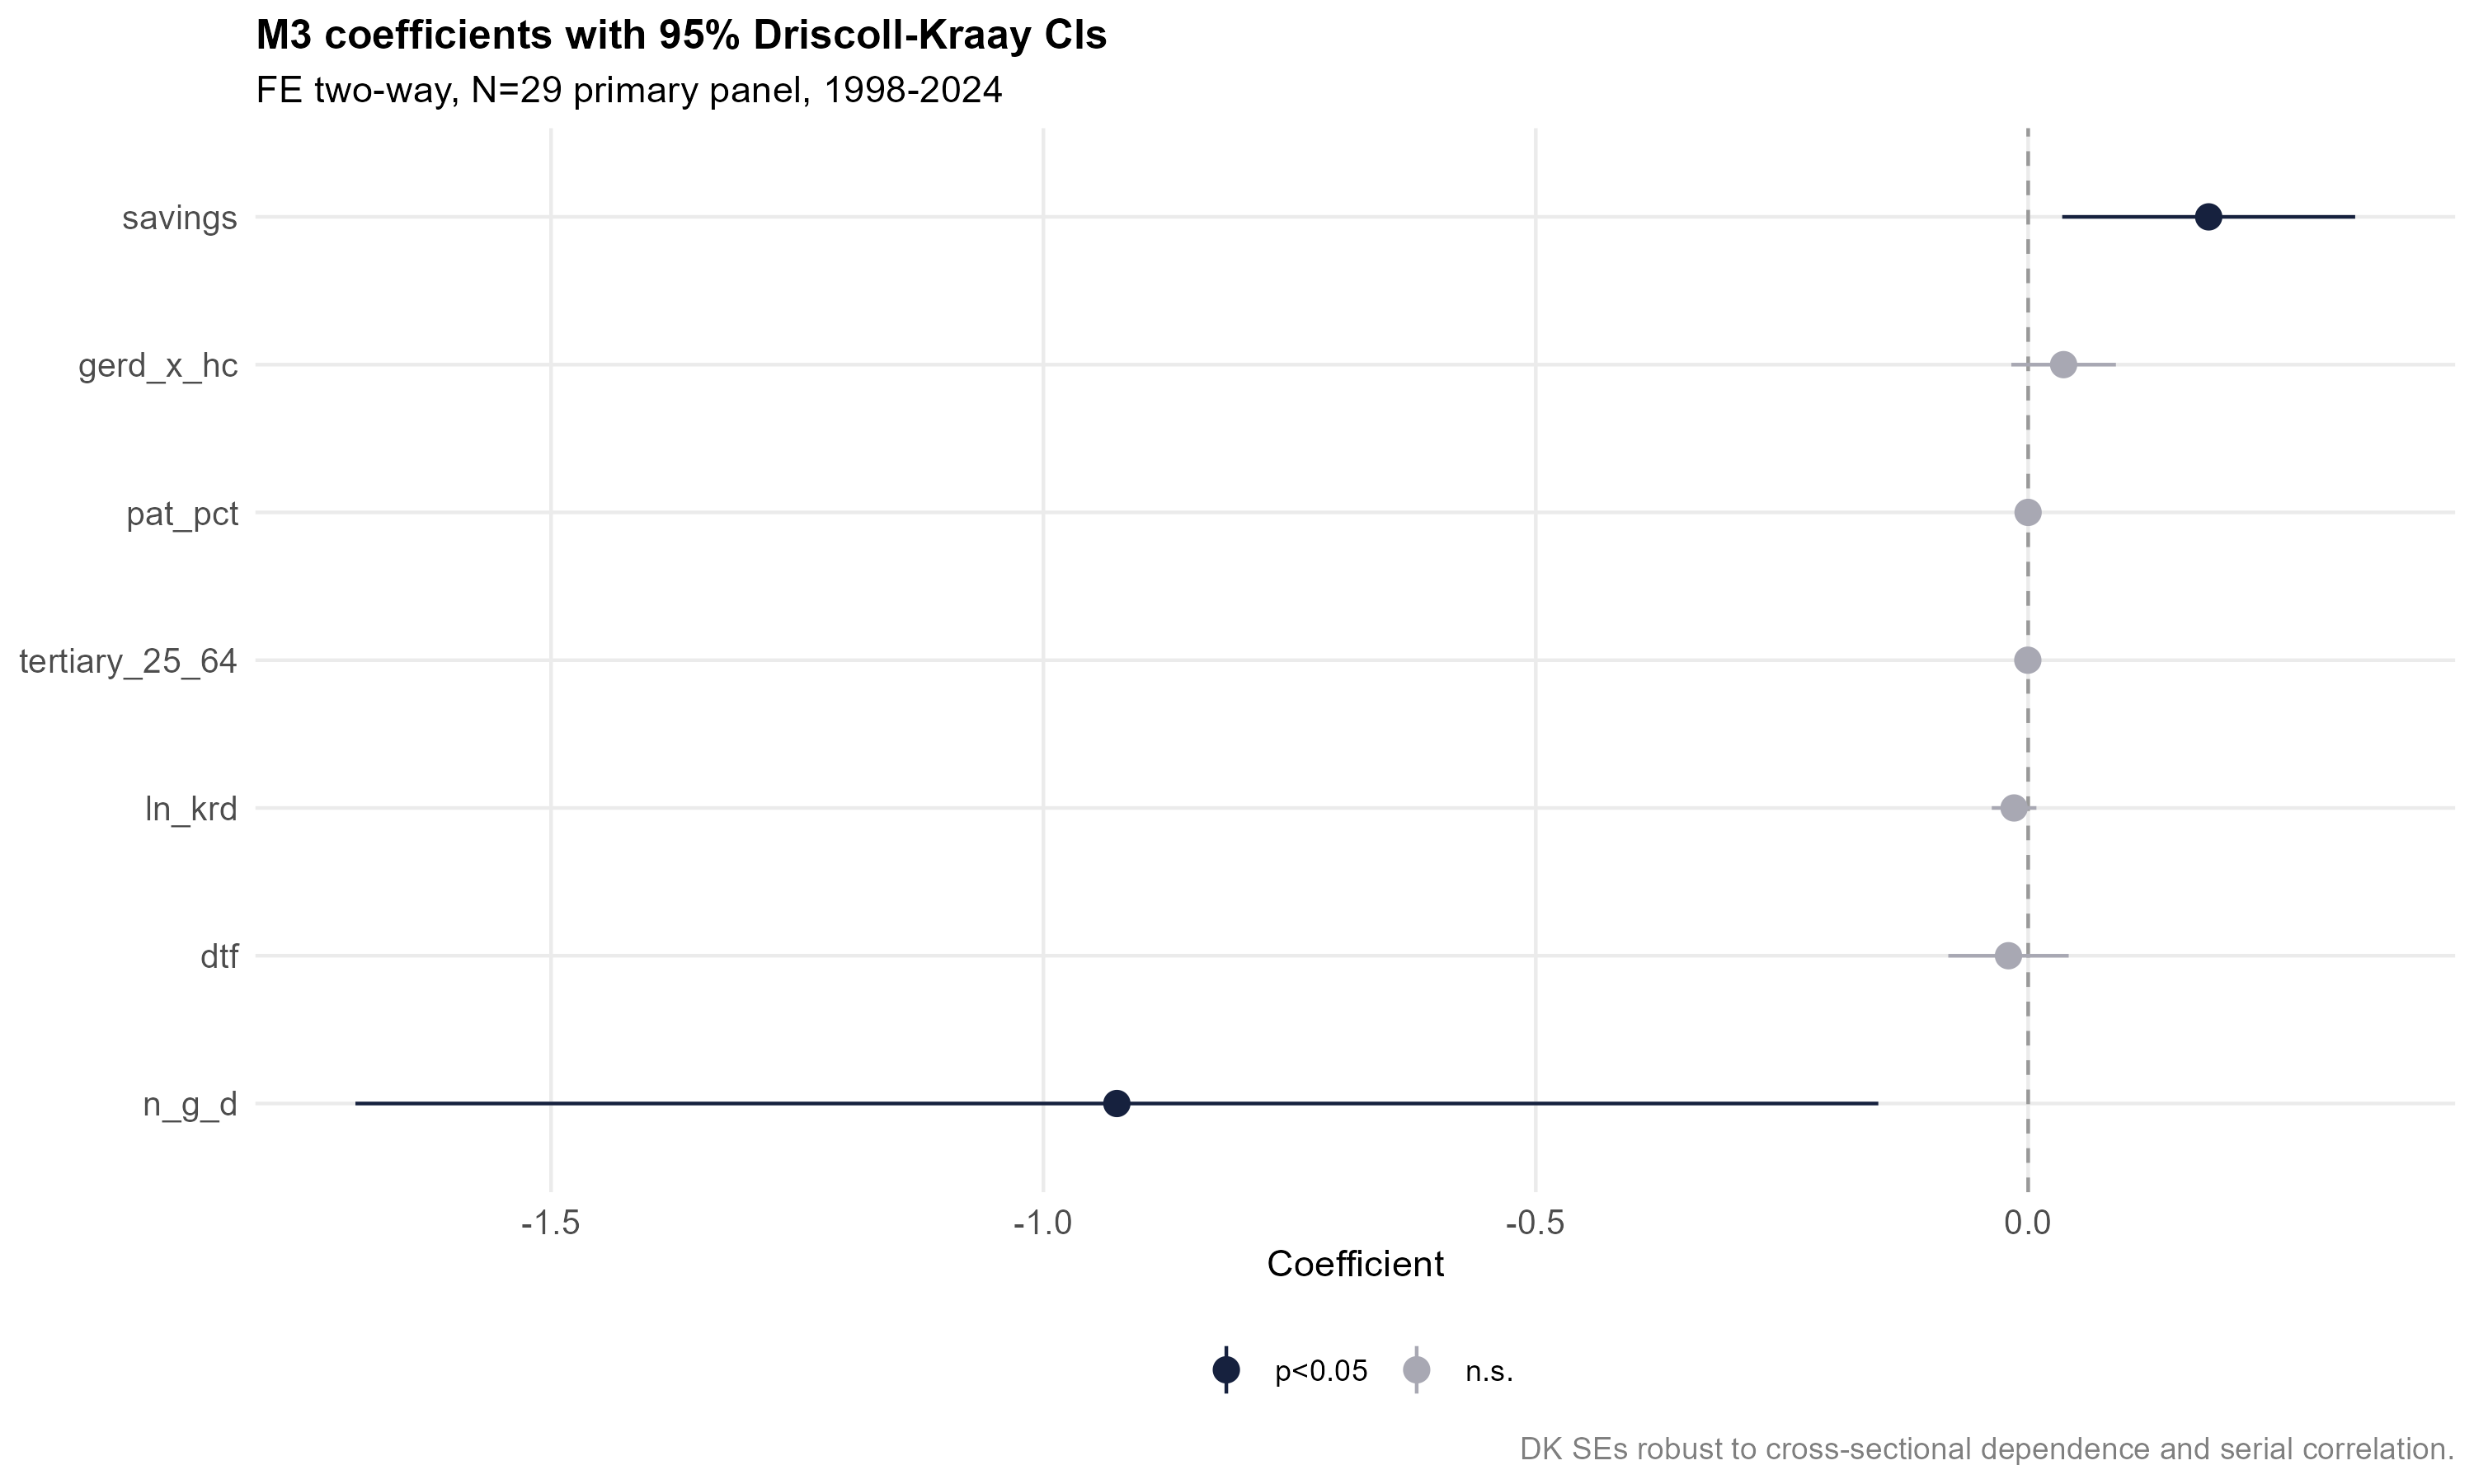
\includegraphics[width=0.95\linewidth]{figures/03_coef_plot_m3} 

}

\caption{Model M3 coefficient plot with 95\% Driscoll--Kraay confidence intervals.}(\#fig:fig-coef)
\end{figure}

\hypertarget{endogeneity-direction}{%
\subsection{Endogeneity Direction}\label{endogeneity-direction}}

The Wu--Hausman test rejects the null of GERD exogeneity (\(p = 0.004\)). The IV coefficient using \(\text{GERD}_{t-2,t-3}\) as instruments (\(F_{\text{first stage}} = 459\), well above the weak-instrument threshold of 10) is \(\hat\beta_{\text{IV}} \approx +0.010\), exceeding the FE estimate of \(-0.003\). Since IV \(>\) FE, the direction of bias is consistent with downward attenuation from classical measurement error (\protect\hyperlink{ref-griliches1979}{Griliches 1979}), not with upward bias from reverse causality. This implies that the FE null is a conservative lower bound on the true coefficient, not an upward-biased one. Figure @ref(fig:fig-iv) illustrates this comparison.

\begin{figure}

{\centering 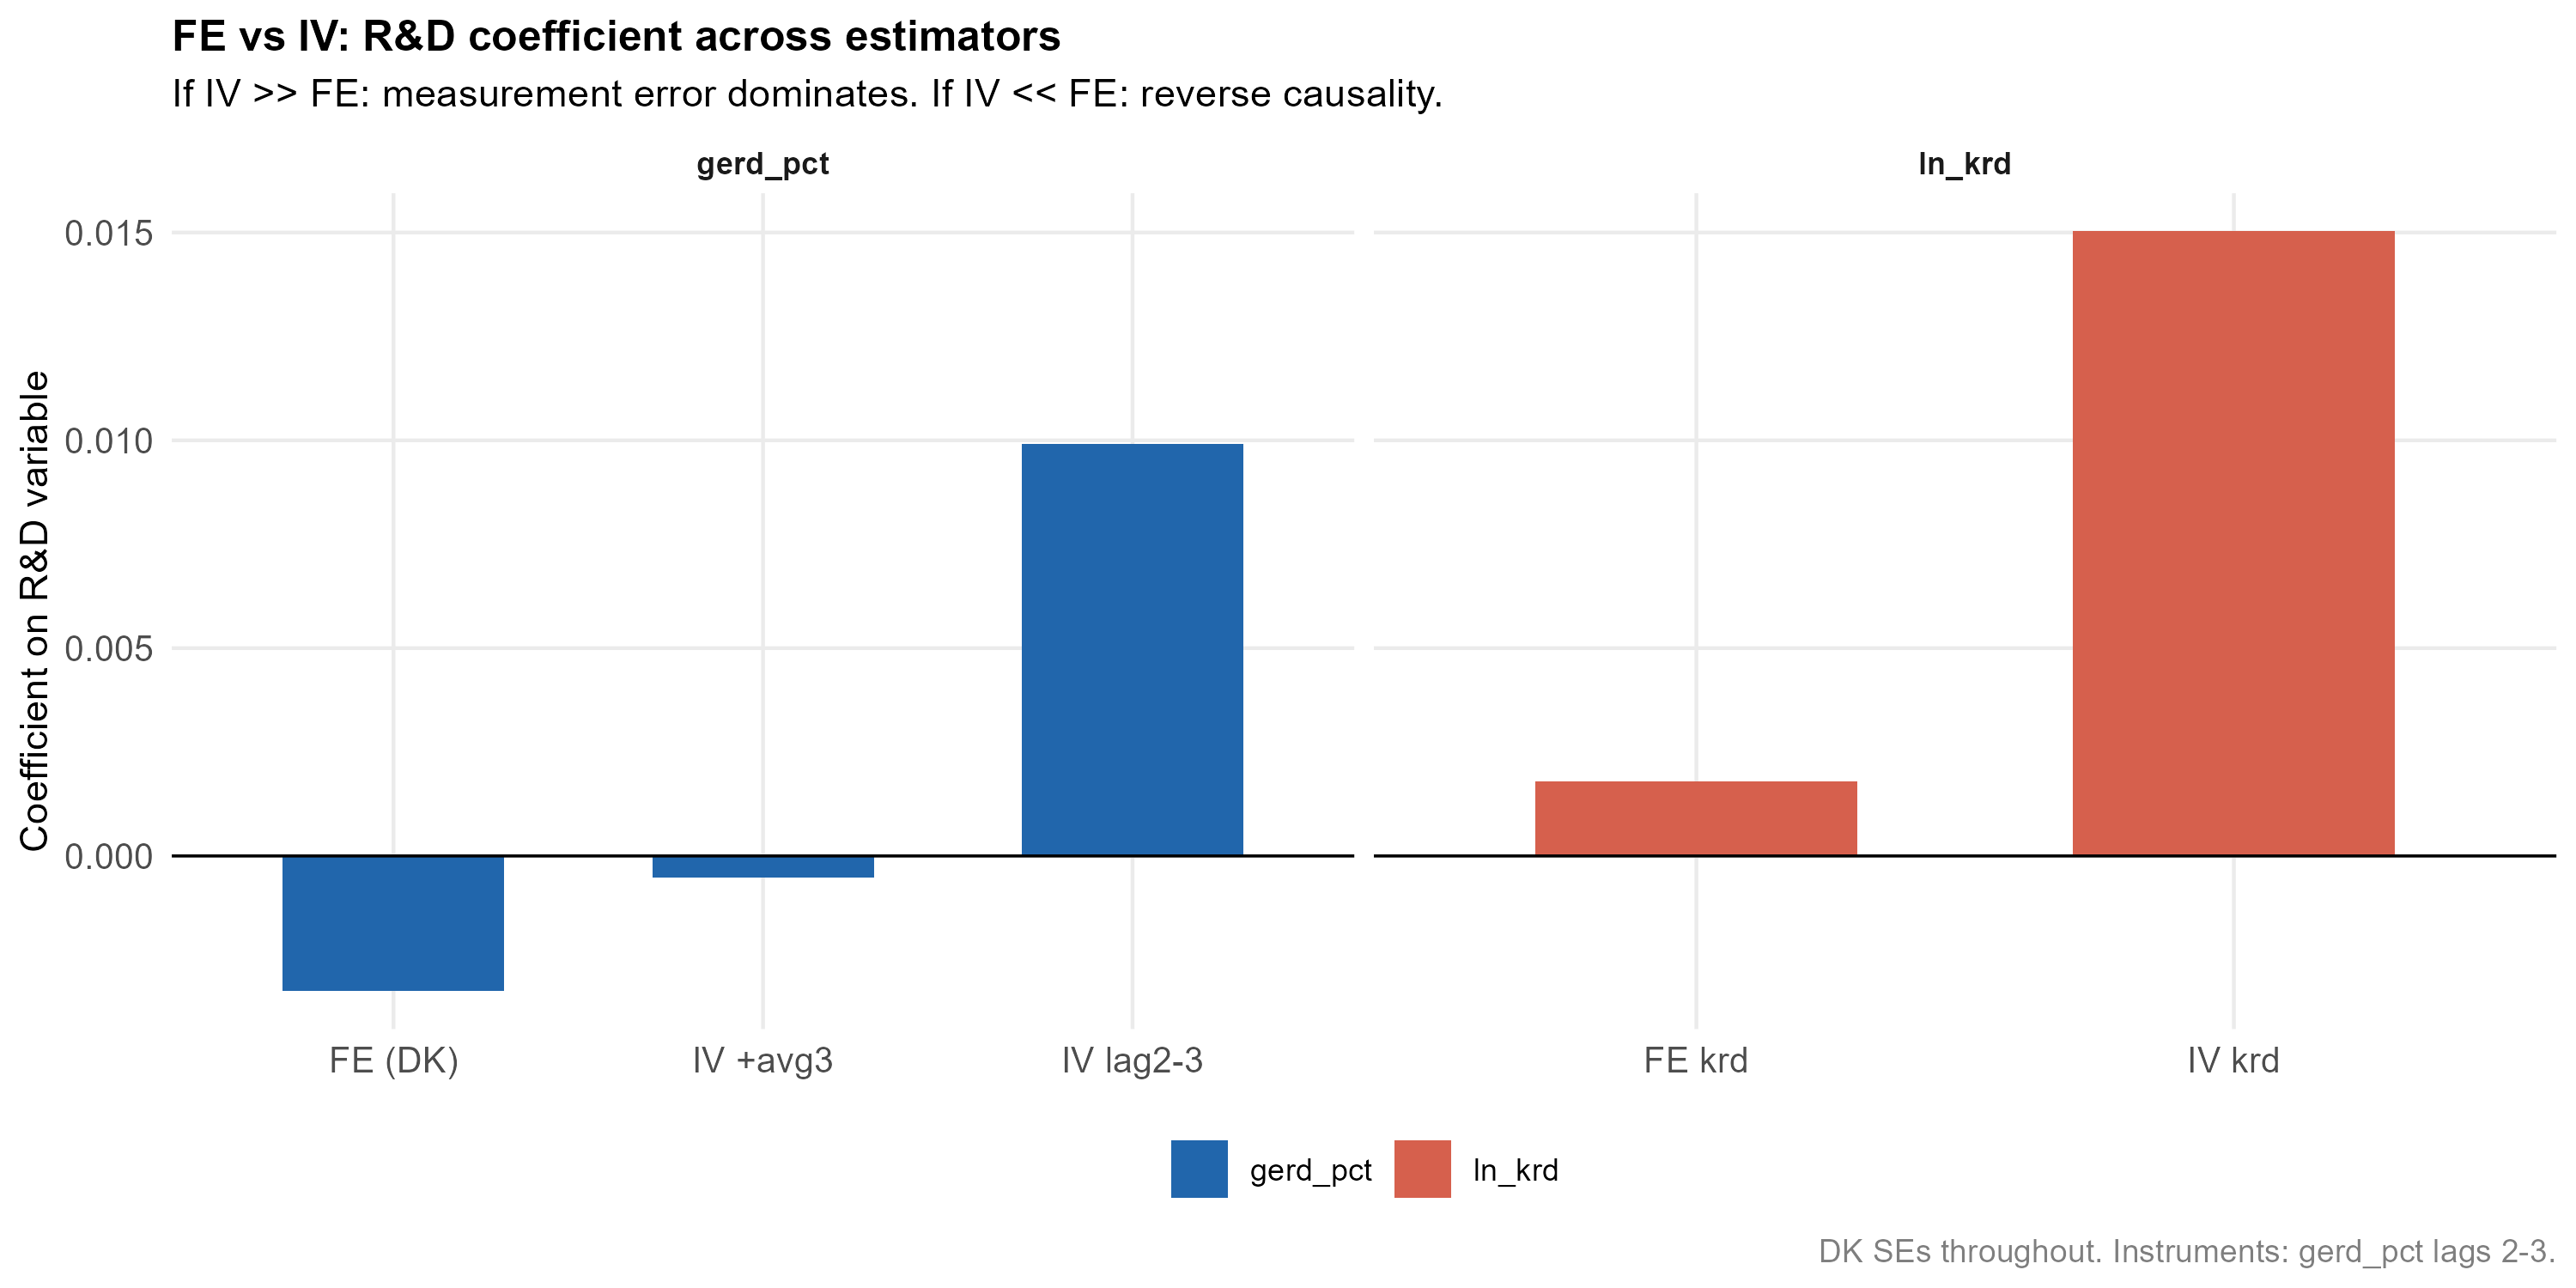
\includegraphics[width=0.95\linewidth]{figures/04_fe_vs_iv} 

}

\caption{FE vs IV coefficient estimates across specifications. IV > FE indicates measurement-error attenuation, not reverse-causality upward bias.}(\#fig:fig-iv)
\end{figure}

\hypertarget{dynamic-effects-local-projections}{%
\subsection{Dynamic Effects: Local Projections}\label{dynamic-effects-local-projections}}

\begin{table}[!h]
\centering
\caption{(\#tab:irf-table)Local projection IRF coefficients: full panel (N=29). Shock = +1pp GERD/GDP.}
\centering
\begin{tabular}[t]{rrrrrr}
\toprule
Horizon $h$ & Coefficient & SE & 90\% CI lo & 90\% CI hi & N obs\\
\midrule
0 & -0.0589 & 0.0329 & -0.1130 & -0.0048 & 683\\
1 & -0.0633 & 0.0422 & -0.1328 & 0.0061 & 654\\
2 & -0.0167 & 0.0384 & -0.0798 & 0.0464 & 625\\
3 & -0.0127 & 0.0432 & -0.0838 & 0.0584 & 596\\
4 & -0.0445 & 0.0404 & -0.1111 & 0.0220 & 567\\
5 & -0.0507 & 0.0381 & -0.1133 & 0.0119 & 538\\
6 & -0.0277 & 0.0396 & -0.0929 & 0.0375 & 509\\
7 & -0.0282 & 0.0348 & -0.0854 & 0.0290 & 480\\
8 & -0.0049 & 0.0375 & -0.0666 & 0.0567 & 451\\
\bottomrule
\multicolumn{6}{l}{\rule{0pt}{1em}\textit{Note:} Two-way FE (country + year), Driscoll--Kraay SEs. Lag controls: s\_\{t-1\}, s\_\{t-2\}, growth\_\{t-1\}, growth\_\{t-2\}.}\\
\end{tabular}
\end{table}

Table @ref(tab:irf-table) and Figure @ref(fig:fig-irf-full) show the impulse response of log GDP per capita to a +1 percentage-point GERD shock in the full panel. The contemporaneous response is small and negative (\(h = 0\): \(\hat\beta = -0.0589\)); no horizon achieves significance at the 90 per cent level beyond \(h = 0\). The typical confidence intervals span approximately \(\pm 0.06\) log-points, leaving substantial statistical uncertainty even at short horizons.

\begin{figure}

{\centering 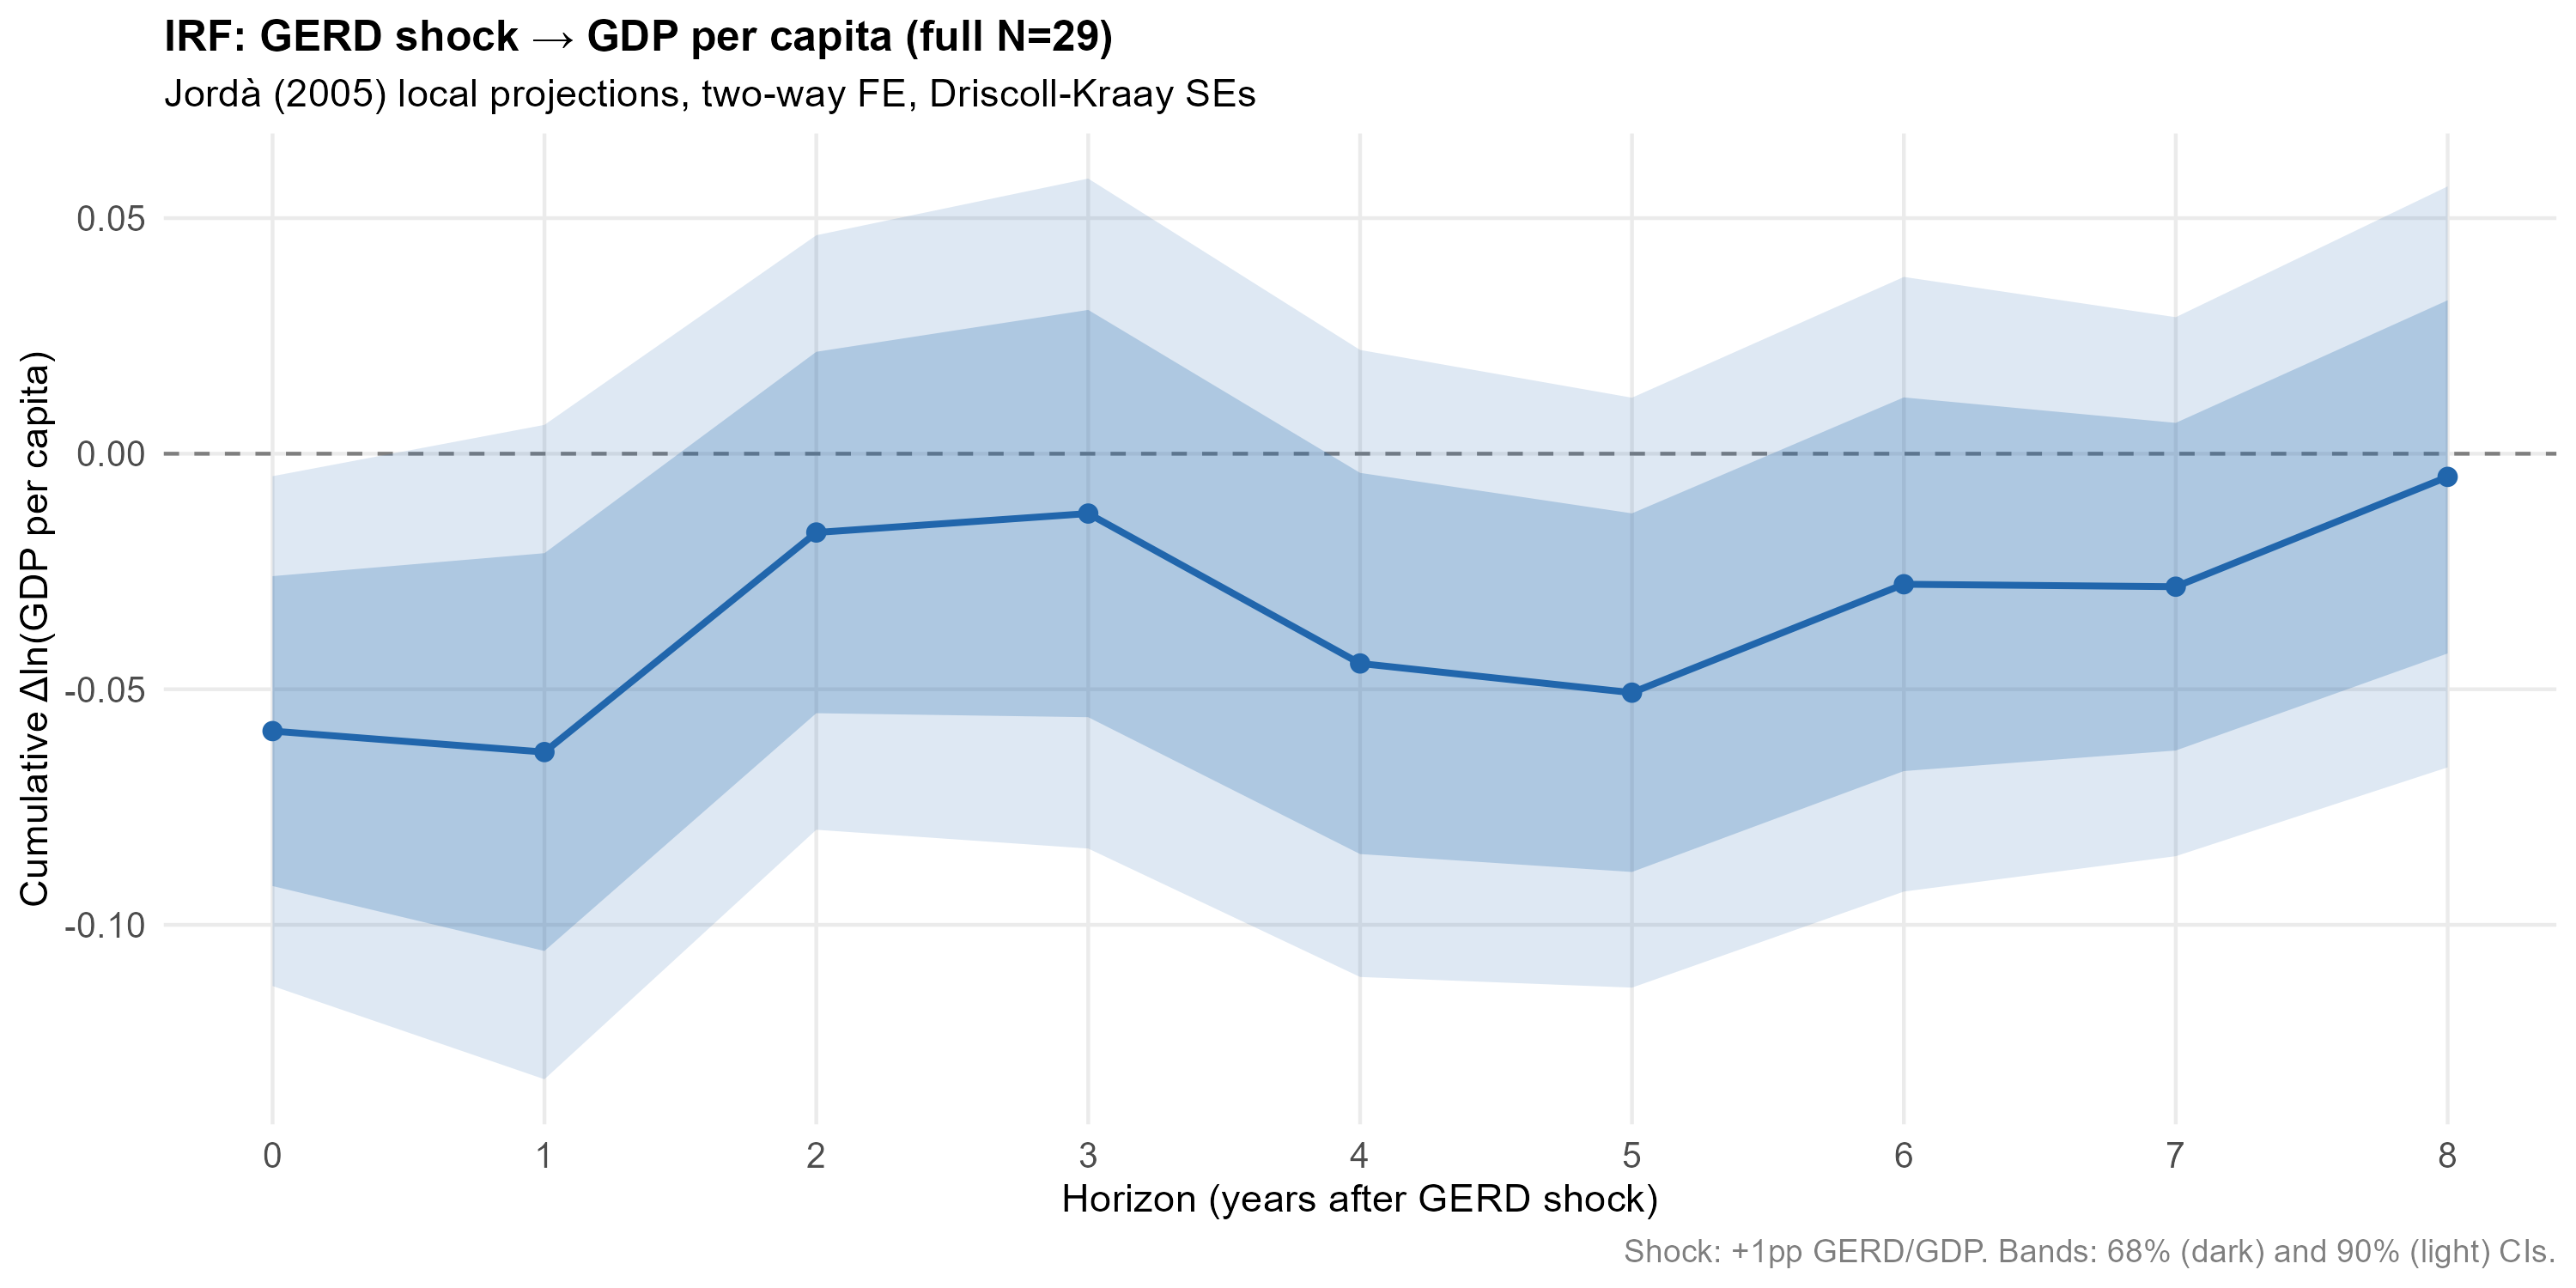
\includegraphics[width=0.95\linewidth]{figures/05_irf_full} 

}

\caption{IRF: GERD shock on cumulative log GDP per capita (full panel, N=29). Bands: 68\% (dark) and 90\% (light).}(\#fig:fig-irf-full)
\end{figure}

The frontier split (Figure @ref(fig:fig-irf-split)) tells a sharply different story. Close-to-frontier economies exhibit a pattern of negative cumulative responses that is statistically significant at the 90 per cent level at horizons \(h = 0, 1, 2, 4, 5, 6, 7\) (peak: \(-0.122\) at \(h = 6\)). Catch-up economies show a positive and rising response that becomes marginally significant only at \(h = 8\) (peak: \(+0.091\)). These two patterns are consistent with the Aghion--Akcigit--Howitt prediction: frontier economies engage in innovation-intensive R\&D that improves the global knowledge stock but generates spillouts to trading partners, while catch-up economies benefit from knowledge absorption on a longer lag.

\begin{figure}

{\centering 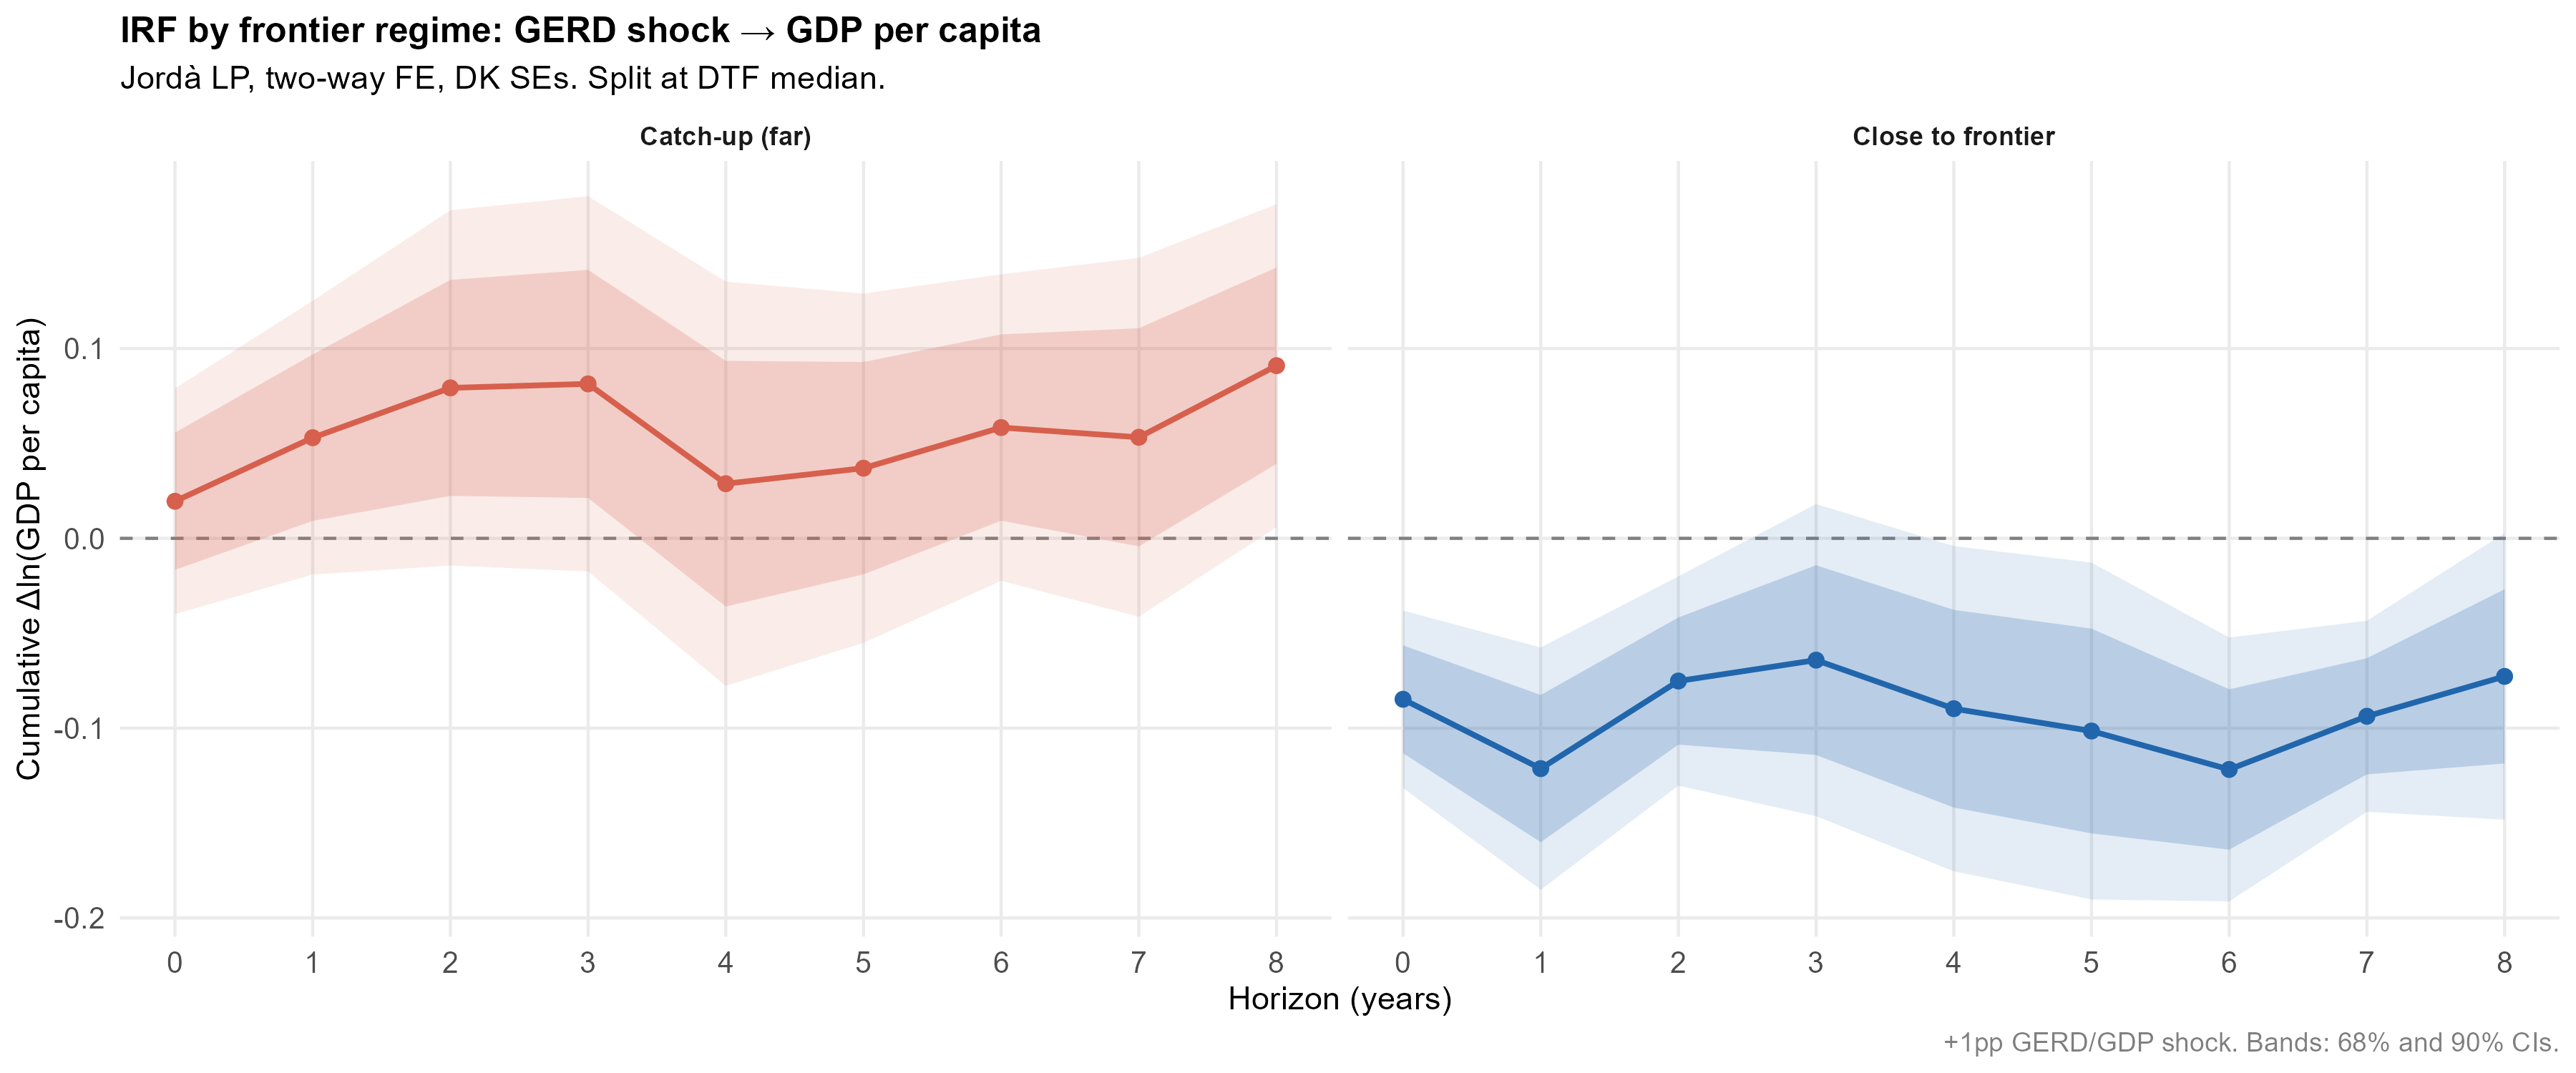
\includegraphics[width=0.95\linewidth]{figures/05_irf_split} 

}

\caption{IRF frontier split: close-to-frontier (blue) vs catch-up (red). Bands: 90\% CI.}(\#fig:fig-irf-split)
\end{figure}

\hypertarget{spatial-spillovers}{%
\subsection{Spatial Spillovers}\label{spatial-spillovers}}

Table @ref(tab:spatial-table) presents the spatial lag-X results under three weight matrices. Direct effects (own-country GERD) remain non-significant across all specifications (\(|\hat\beta| < 0.007\)). Indirect effects (neighbours' GERD) are similarly imprecisely estimated: \(W_1\) gives \(\hat\theta = +0.012\) (SE \(= 0.038\), n.s.); \(W_2\) gives \(\hat\theta = +0.0004\) (n.s.); \(W_3\) gives \(\hat\theta = -0.037\) (n.s.). The full SDM via ML estimation (splm, \(N = 29\), \(T = 20\) balanced) returns a spatial autoregressive coefficient \(\lambda = 0.107\) (\(p = 0.325\)), indicating that cross-country growth co-movement is weak once two-way fixed effects absorb common shocks. Moran's \(I = -0.005\) (\(p = 0.22\)) on FE residuals in the most recent year confirms no residual spatial clustering.

\begin{table}[!h]
\centering
\caption{(\#tab:spatial-table)Spatial Durbin Model-X: direct, indirect, and total effects of GERD on growth.}
\centering
\begin{tabular}[t]{lrrrr}
\toprule
Specification & Direct $\hat{\beta}$ & Indirect $\hat{\theta}$ & Total $\hat{\beta}+\hat{\theta}$ & N obs\\
\midrule
Baseline FE & -0.0033 & NA & NA & 734\\
W1 (inv-dist) & -0.0037 & 0.0116 & 0.0079 & 711\\
W2 (contiguity) & -0.0043 & 0.0004 & -0.0039 & 711\\
W3 (income-prox) & -0.0064 & -0.0367 & -0.0431 & 711\\
\bottomrule
\multicolumn{5}{l}{\rule{0pt}{1em}\textit{Note:} Two-way FE, Driscoll--Kraay SEs. No coefficient is significant at 10% level.}\\
\end{tabular}
\end{table}

\begin{figure}

{\centering 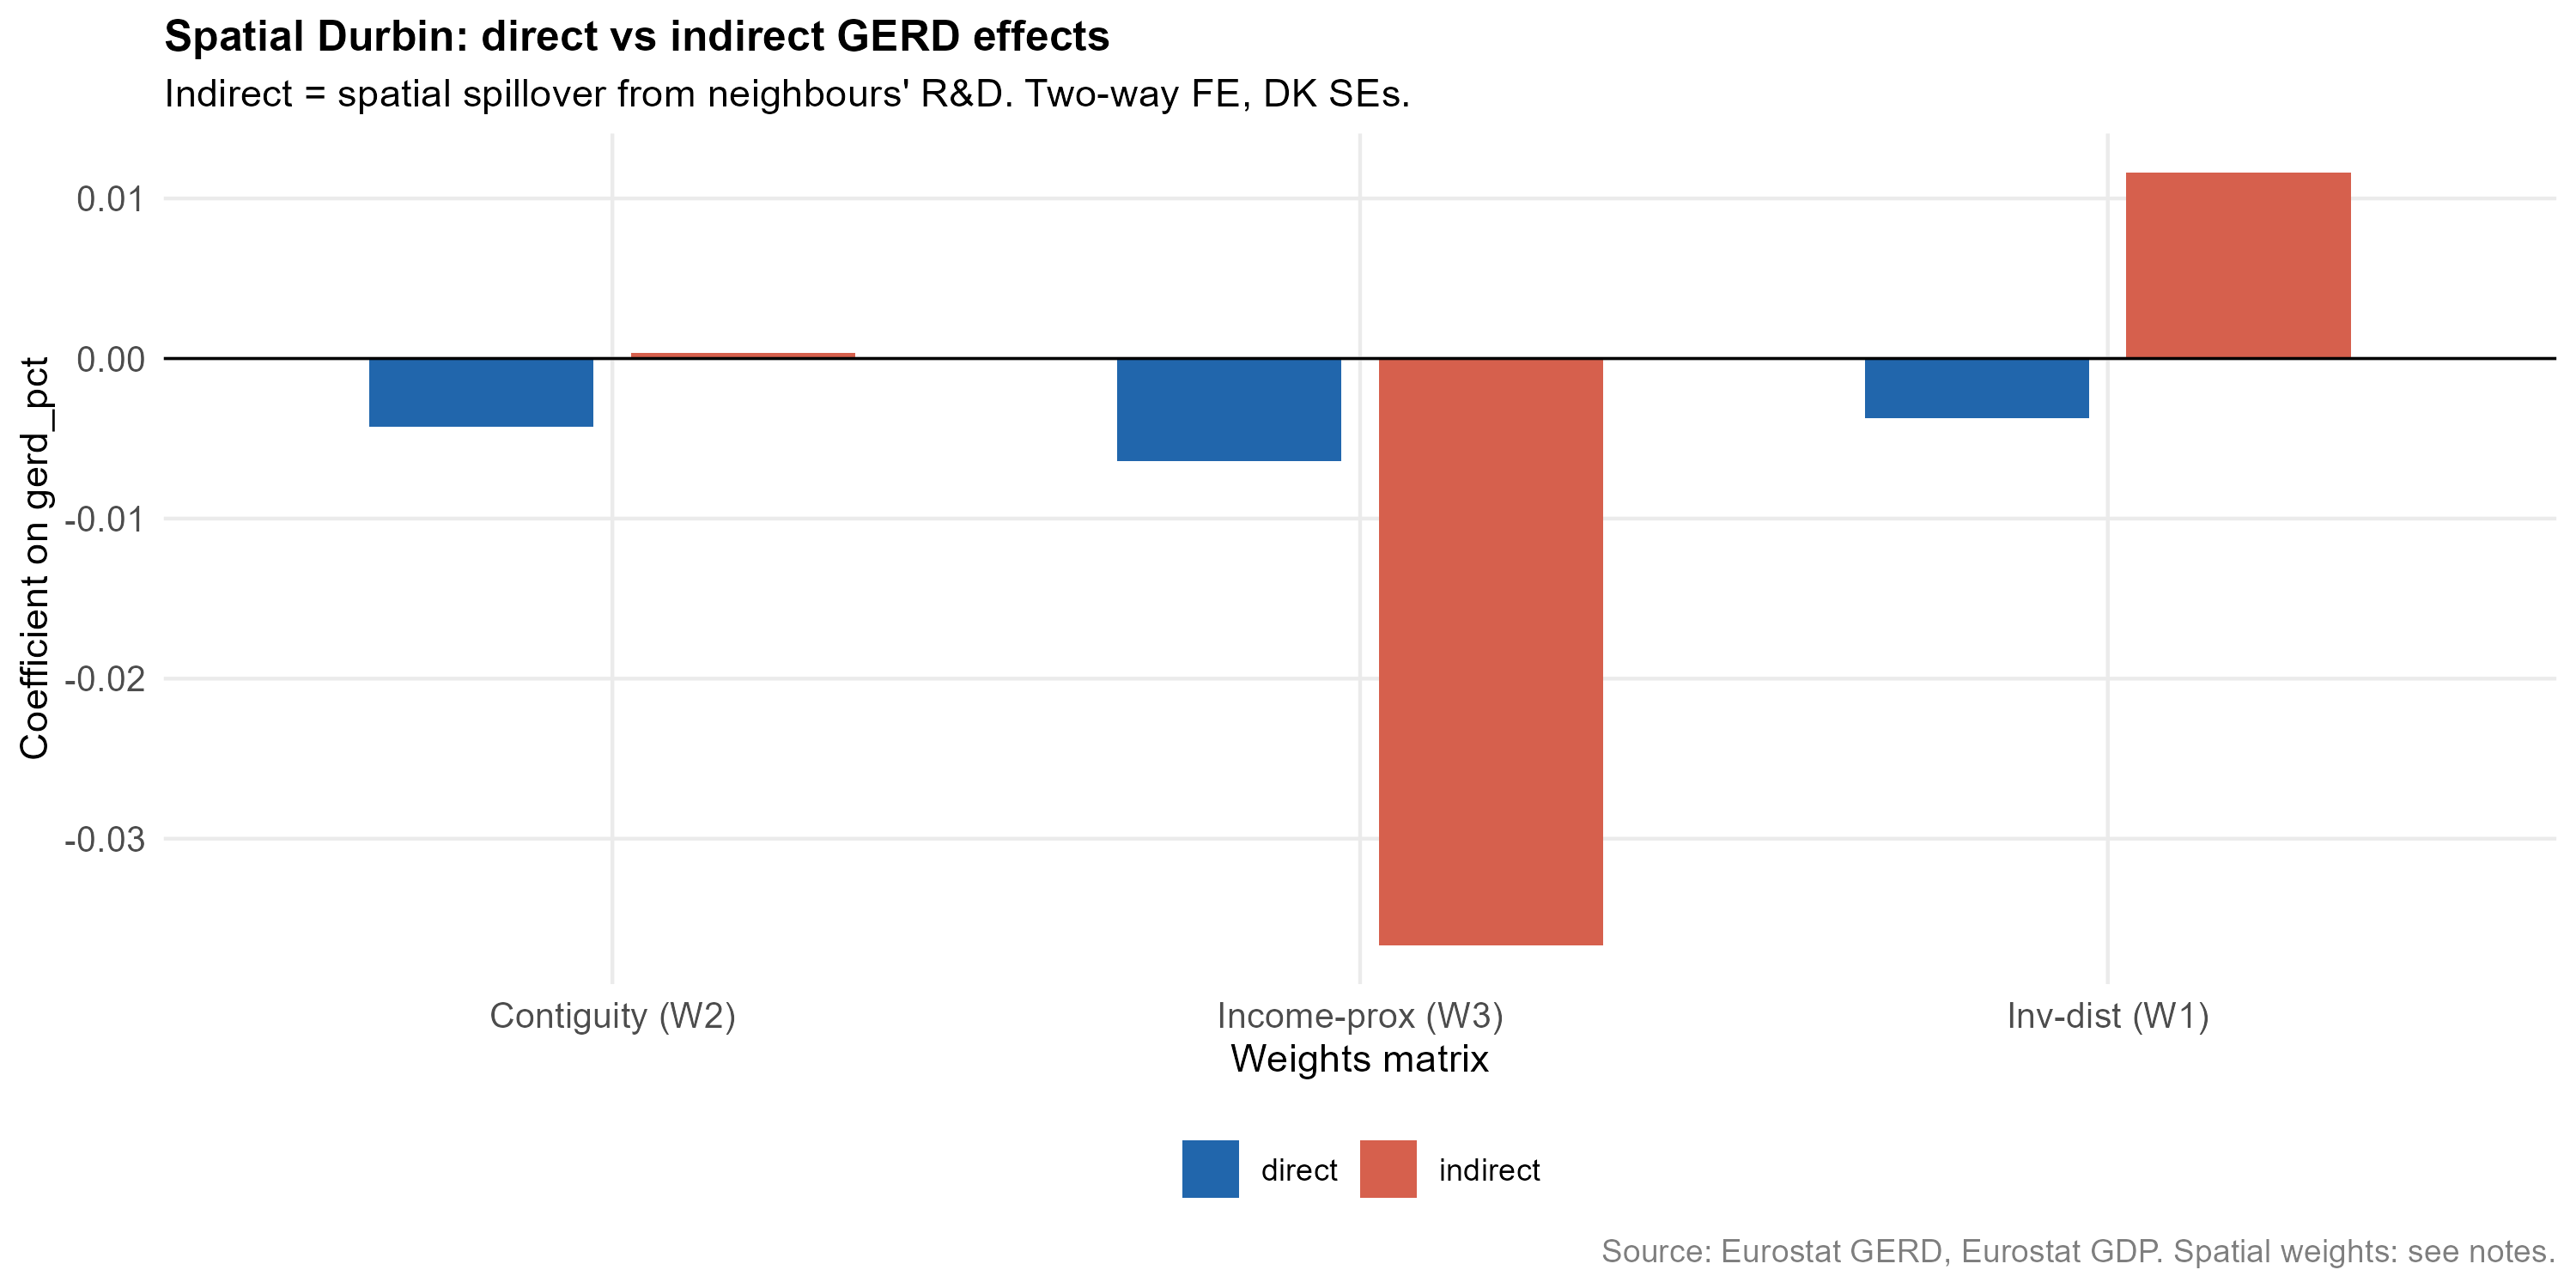
\includegraphics[width=0.95\linewidth]{figures/06_spatial_effects} 

}

\caption{Spatial Durbin direct vs indirect GERD effects by weight matrix. None is statistically significant.}(\#fig:fig-spatial)
\end{figure}

\hypertarget{heterogeneous-treatment-effects}{%
\subsection{Heterogeneous Treatment Effects}\label{heterogeneous-treatment-effects}}

\begin{table}[!h]
\centering
\caption{(\#tab:hte-table)ATE estimates: FE baseline, DML-OLS, DML-Ridge, Causal Forest.}
\centering
\begin{tabular}[t]{lrrrr}
\toprule
Estimator & $\hat{\theta}$ & SE & 90\% CI lo & 90\% CI hi\\
\midrule
DML-OLS & -0.01011 & 0.0067 & -0.02113 & 9e-04\\
DML-Ridge & -0.01064 & 0.00686 & -0.02194 & 0.00065\\
Causal Forest ATE & 0.00364 & 0.01011 & -0.01299 & 0.02028\\
FE (DK) Stage03 & -0.00631 & --- & --- & ---\\
\bottomrule
\multicolumn{5}{l}{\rule{0pt}{1em}\textit{Note:} DML: 5-fold country-blocked cross-fitting. CF: 3,000 trees, country clusters, honest splitting.}\\
\end{tabular}
\end{table}

Table @ref(tab:hte-table) shows that all estimators return an average treatment effect that is not significantly different from zero: DML-Ridge gives \(\hat\theta = -0.0106\) (SE \(= 0.007\), \(t = -1.55\)); the causal forest ATE is \(+0.004\) (SE \(= 0.010\)). The consistency of the null across parametric FE, semiparametric DML, and nonparametric causal forest is strong evidence against a significant average GERD--growth effect.

CATE heterogeneity is modest but economically interpretable. The interquartile range of estimated CATEs is \([-0.013, +0.012]\), a spread of approximately 2.5 percentage points around zero. Figure @ref(fig:fig-cate) plots CATE against distance to frontier: there is a weak positive slope (further-from-frontier countries tend to have higher estimated CATEs), consistent with the LP frontier-split result. However, the best linear projection of CATE on \(\text{dtf}\) and \(\ln K\) fails to reject linearity zero (\(t < 0.3\), \(p > 0.77\)), cautioning against strong heterogeneity claims at this sample size.

Variable importance (Figure @ref(fig:fig-vi)) shows that \(n + g + \delta\) (21.5\%), savings (19.0\%), and institutional quality (18.2\%) drive most of the forest's splitting decisions---the same factor-accumulation variables that dominate the parametric models. Distance to frontier ranks fifth (10.1\%), below human capital (12.3\%) and knowledge stock (11.3\%).

\begin{figure}

{\centering 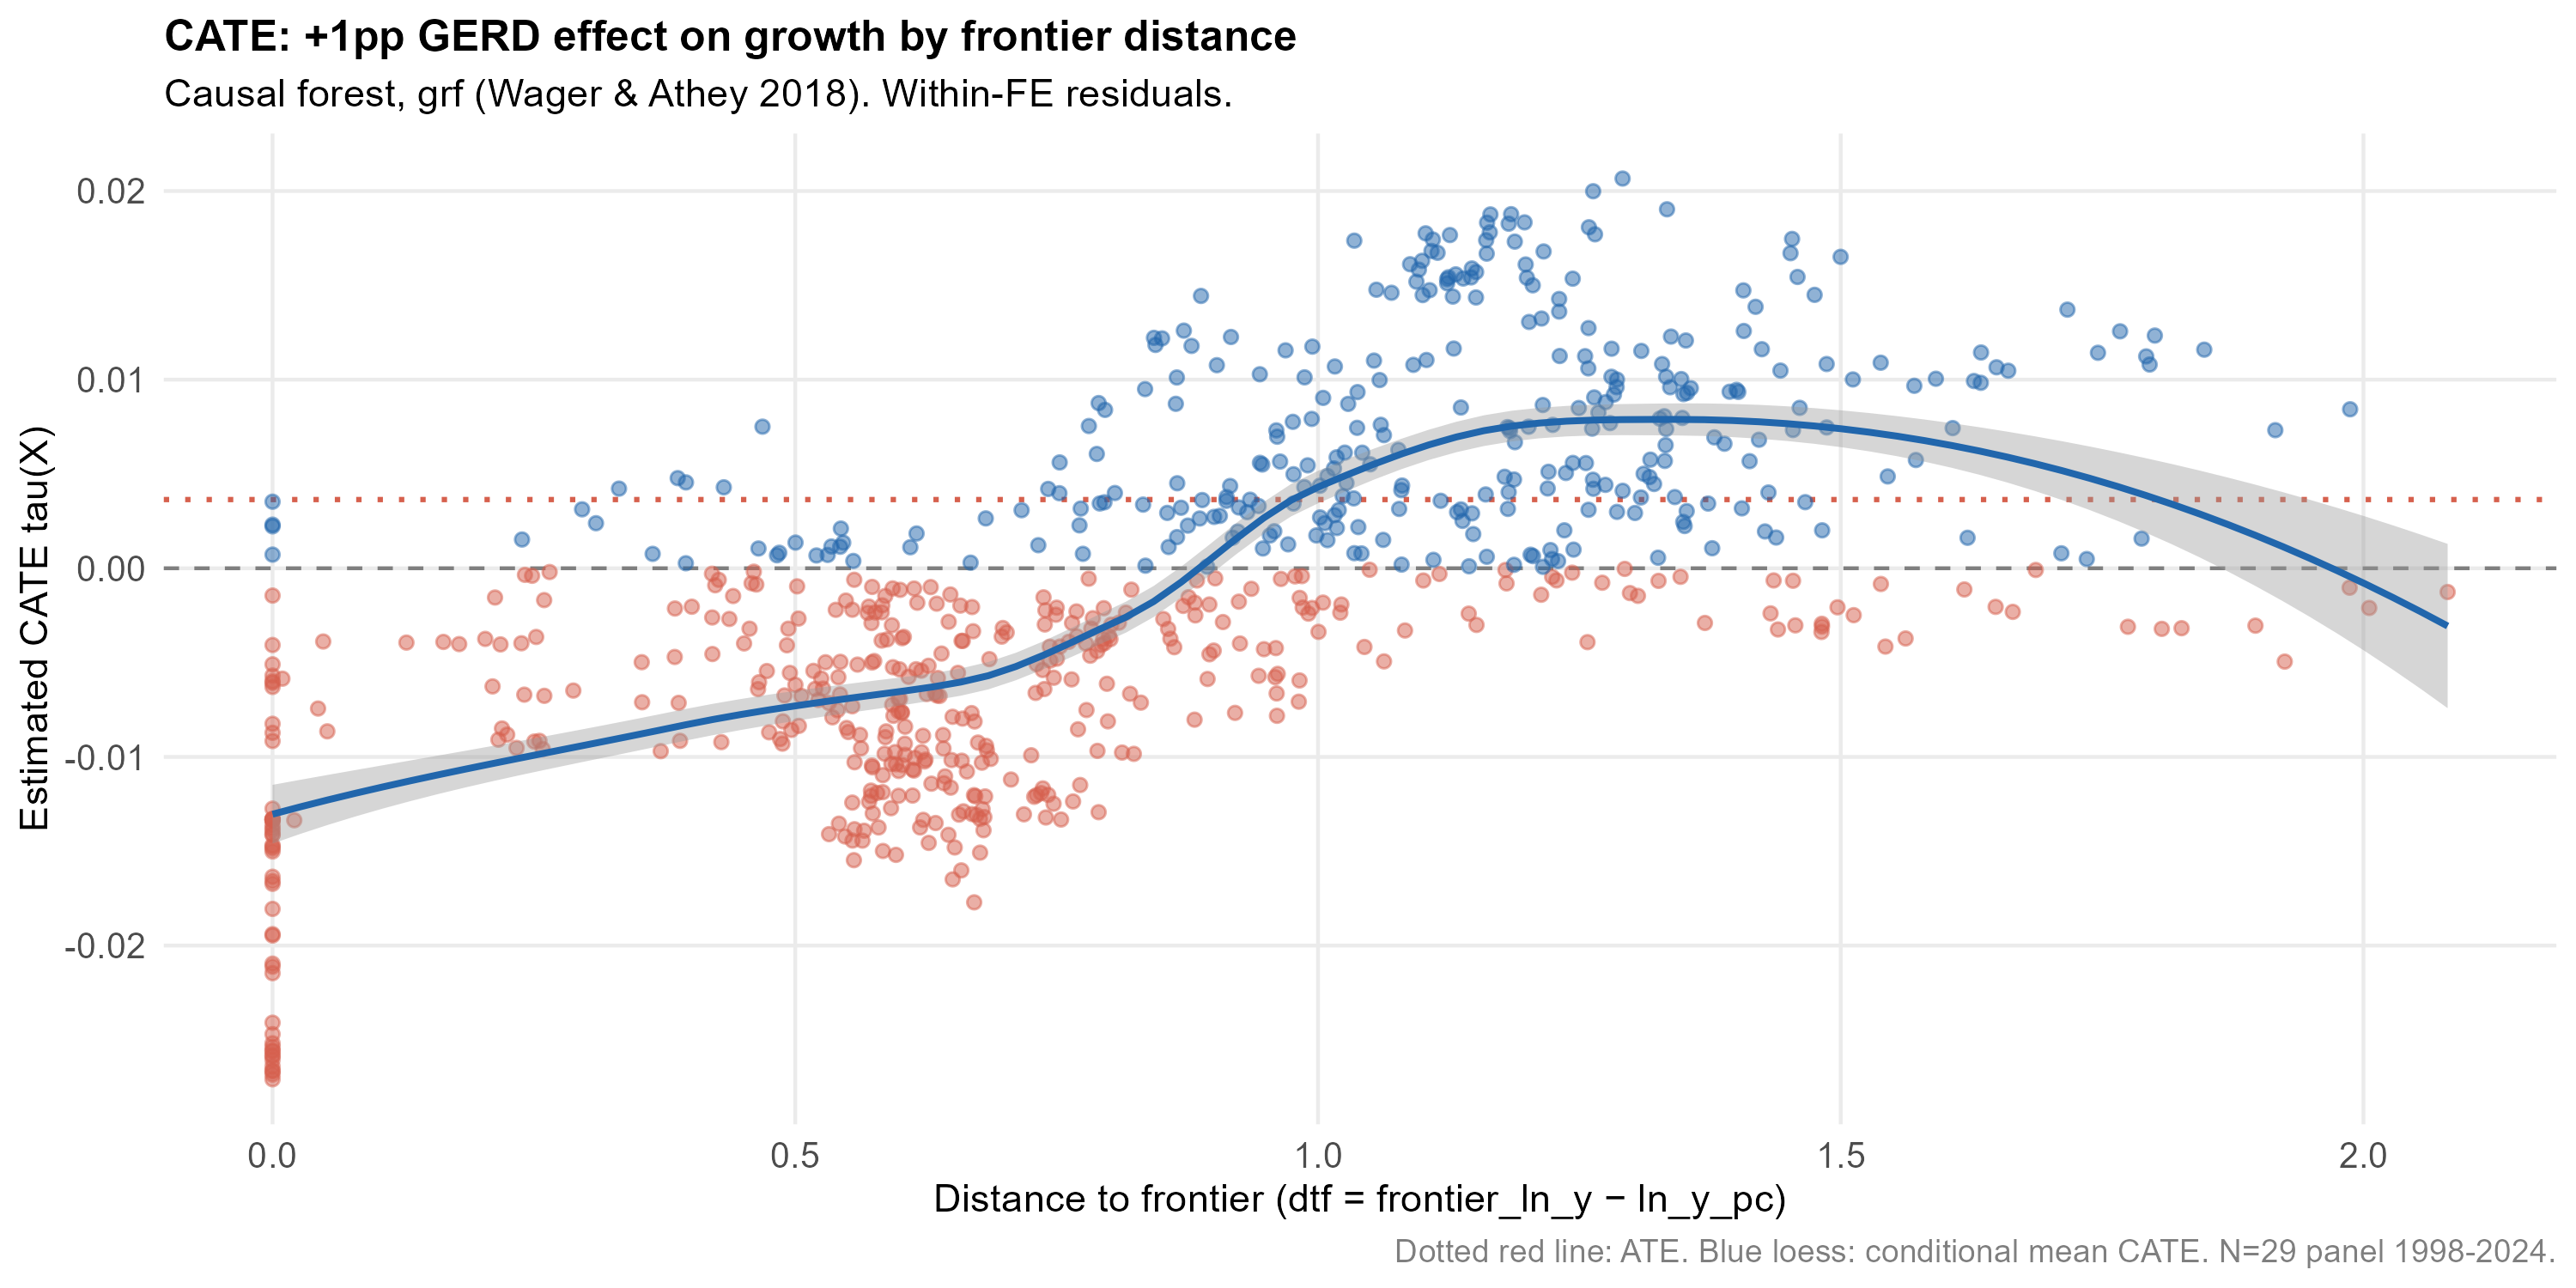
\includegraphics[width=0.95\linewidth]{figures/07_cate_dtf} 

}

\caption{Causal forest CATE estimates vs distance to frontier. Loess smoother. Dotted = ATE.}(\#fig:fig-cate)
\end{figure}

\begin{figure}

{\centering 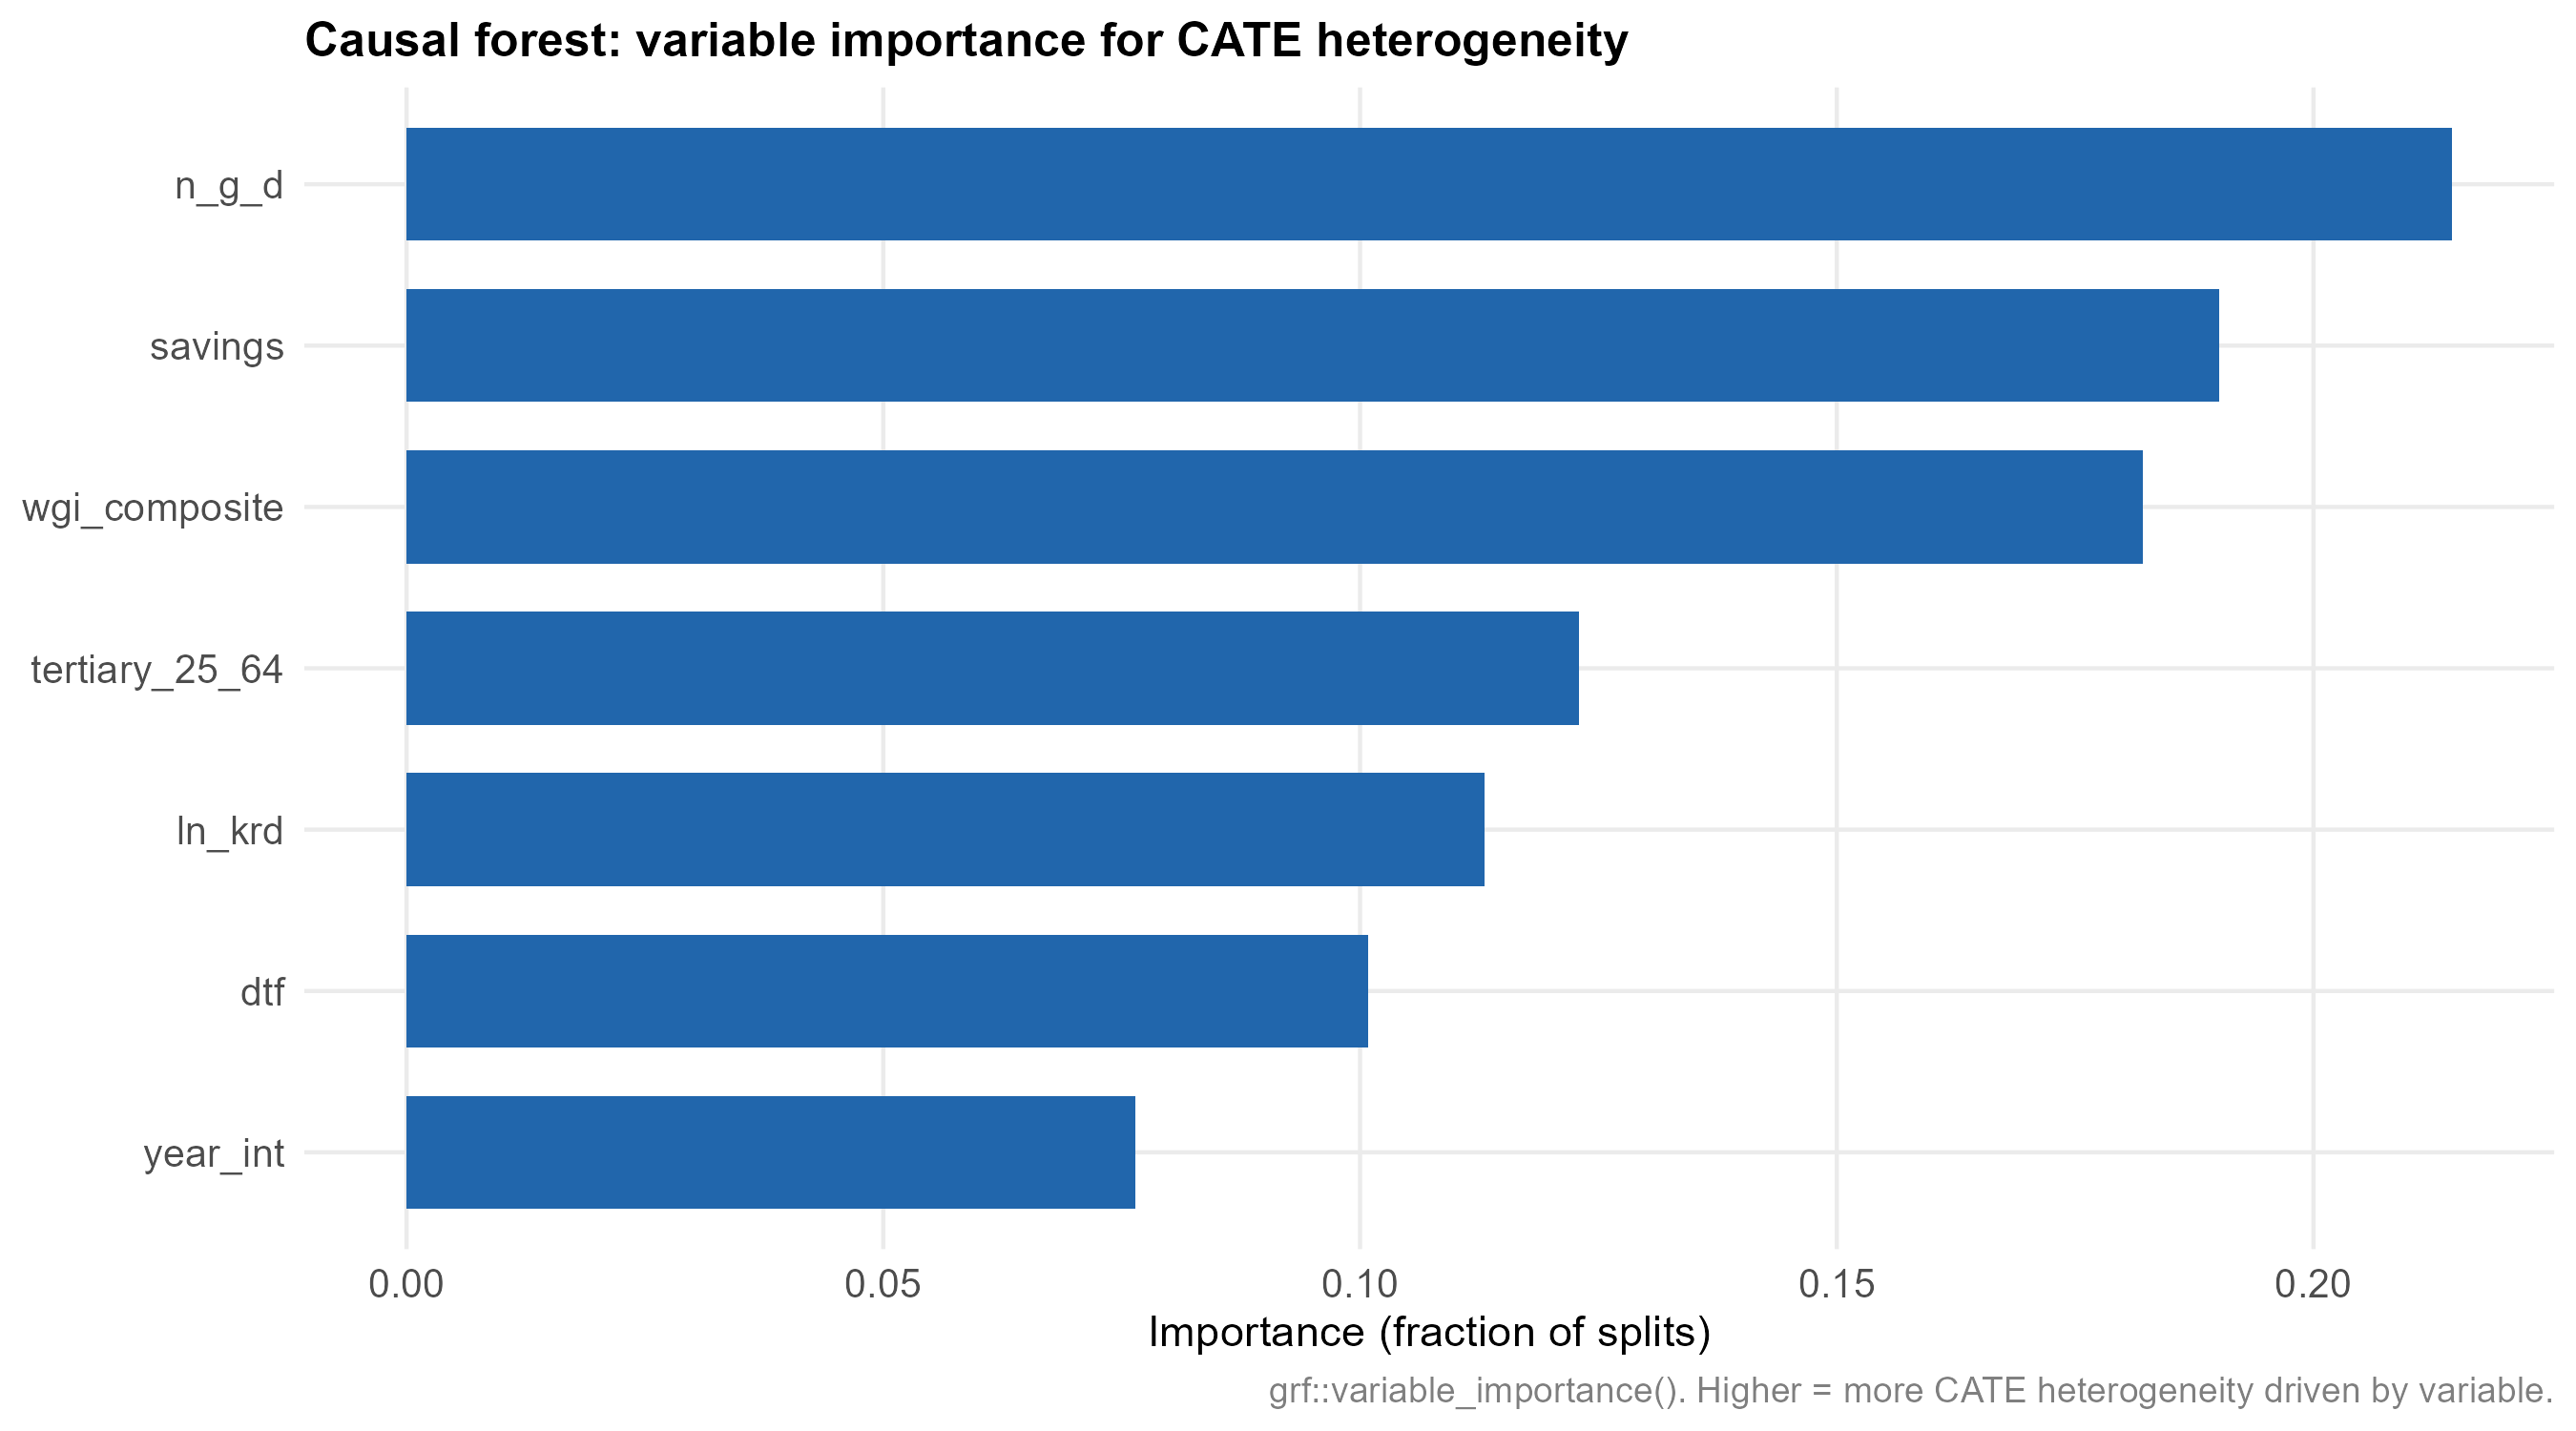
\includegraphics[width=0.95\linewidth]{figures/07_var_importance} 

}

\caption{Causal forest variable importance. Higher = more splits on that variable.}(\#fig:fig-vi)
\end{figure}

\hypertarget{country-typology}{%
\subsection{Country Typology}\label{country-typology}}

Both the silhouette criterion and the gap statistic select \(k = 2\) as the optimal number of clusters (average silhouette \(= 0.486\); gap \(= 0.187\), both largest at \(k = 2\)). Table @ref(tab:cluster-table) reports the cluster profiles.

\begin{table}[!h]
\centering
\caption{(\#tab:cluster-table)K-means cluster profiles (k=2): country means.}
\centering
\begin{tabular}[t]{lrrrrrr}
\toprule
Cluster & GERD \% & ln $K$ & DTF & WGI & HC \% & Savings\\
\midrule
Cluster 1 (n=13) & 2.361 & 2.644 & 0.456 & 26.032 & 34.218 & 0.268\\
Cluster 2 (n=15) & 0.943 & 1.602 & 1.128 & 12.154 & 25.027 & 0.200\\
\bottomrule
\multicolumn{7}{l}{\rule{0pt}{1em}\textit{Note:} 6-feature K-means (nstart=50, set.seed(42)). Silhouette and gap statistics both select k=2.}\\
\end{tabular}
\end{table}

\textbf{Cluster 1 -- Innovation Leaders} (13 countries: AT, BE, CH, DE, DK, FI, FR, IE, IS, LU, NL, NO, SE): Mean GERD \(= 2.36\%\), mean \(\text{dtf} = 0.46\), WGI \(= 26.0\). These are high-R\&D, near-frontier, well-governed economies. Their Stage 07 mean CATE \(= -0.008\), consistent with the LP finding of persistent negative direct effects.

\textbf{Cluster 2 -- Convergence Economies} (15 countries: BG, CY, CZ, EE, ES, GR, HR, HU, IT, LT, LV, MT, PL, PT, SK): Mean GERD \(= 0.94\%\), mean \(\text{dtf} = 1.13\), WGI \(= 12.2\). These are low-R\&D, distant-from-frontier economies. Their Stage 07 mean CATE \(= +0.005\), consistent with the LP catch-up positive response.

Crucially, the cluster assignment reproduces the thesis's k=2 grouping exactly on the extended feature set (same 13/15 country split), validating the earlier typology while grounding it in a richer conceptual basis.

\begin{figure}

{\centering 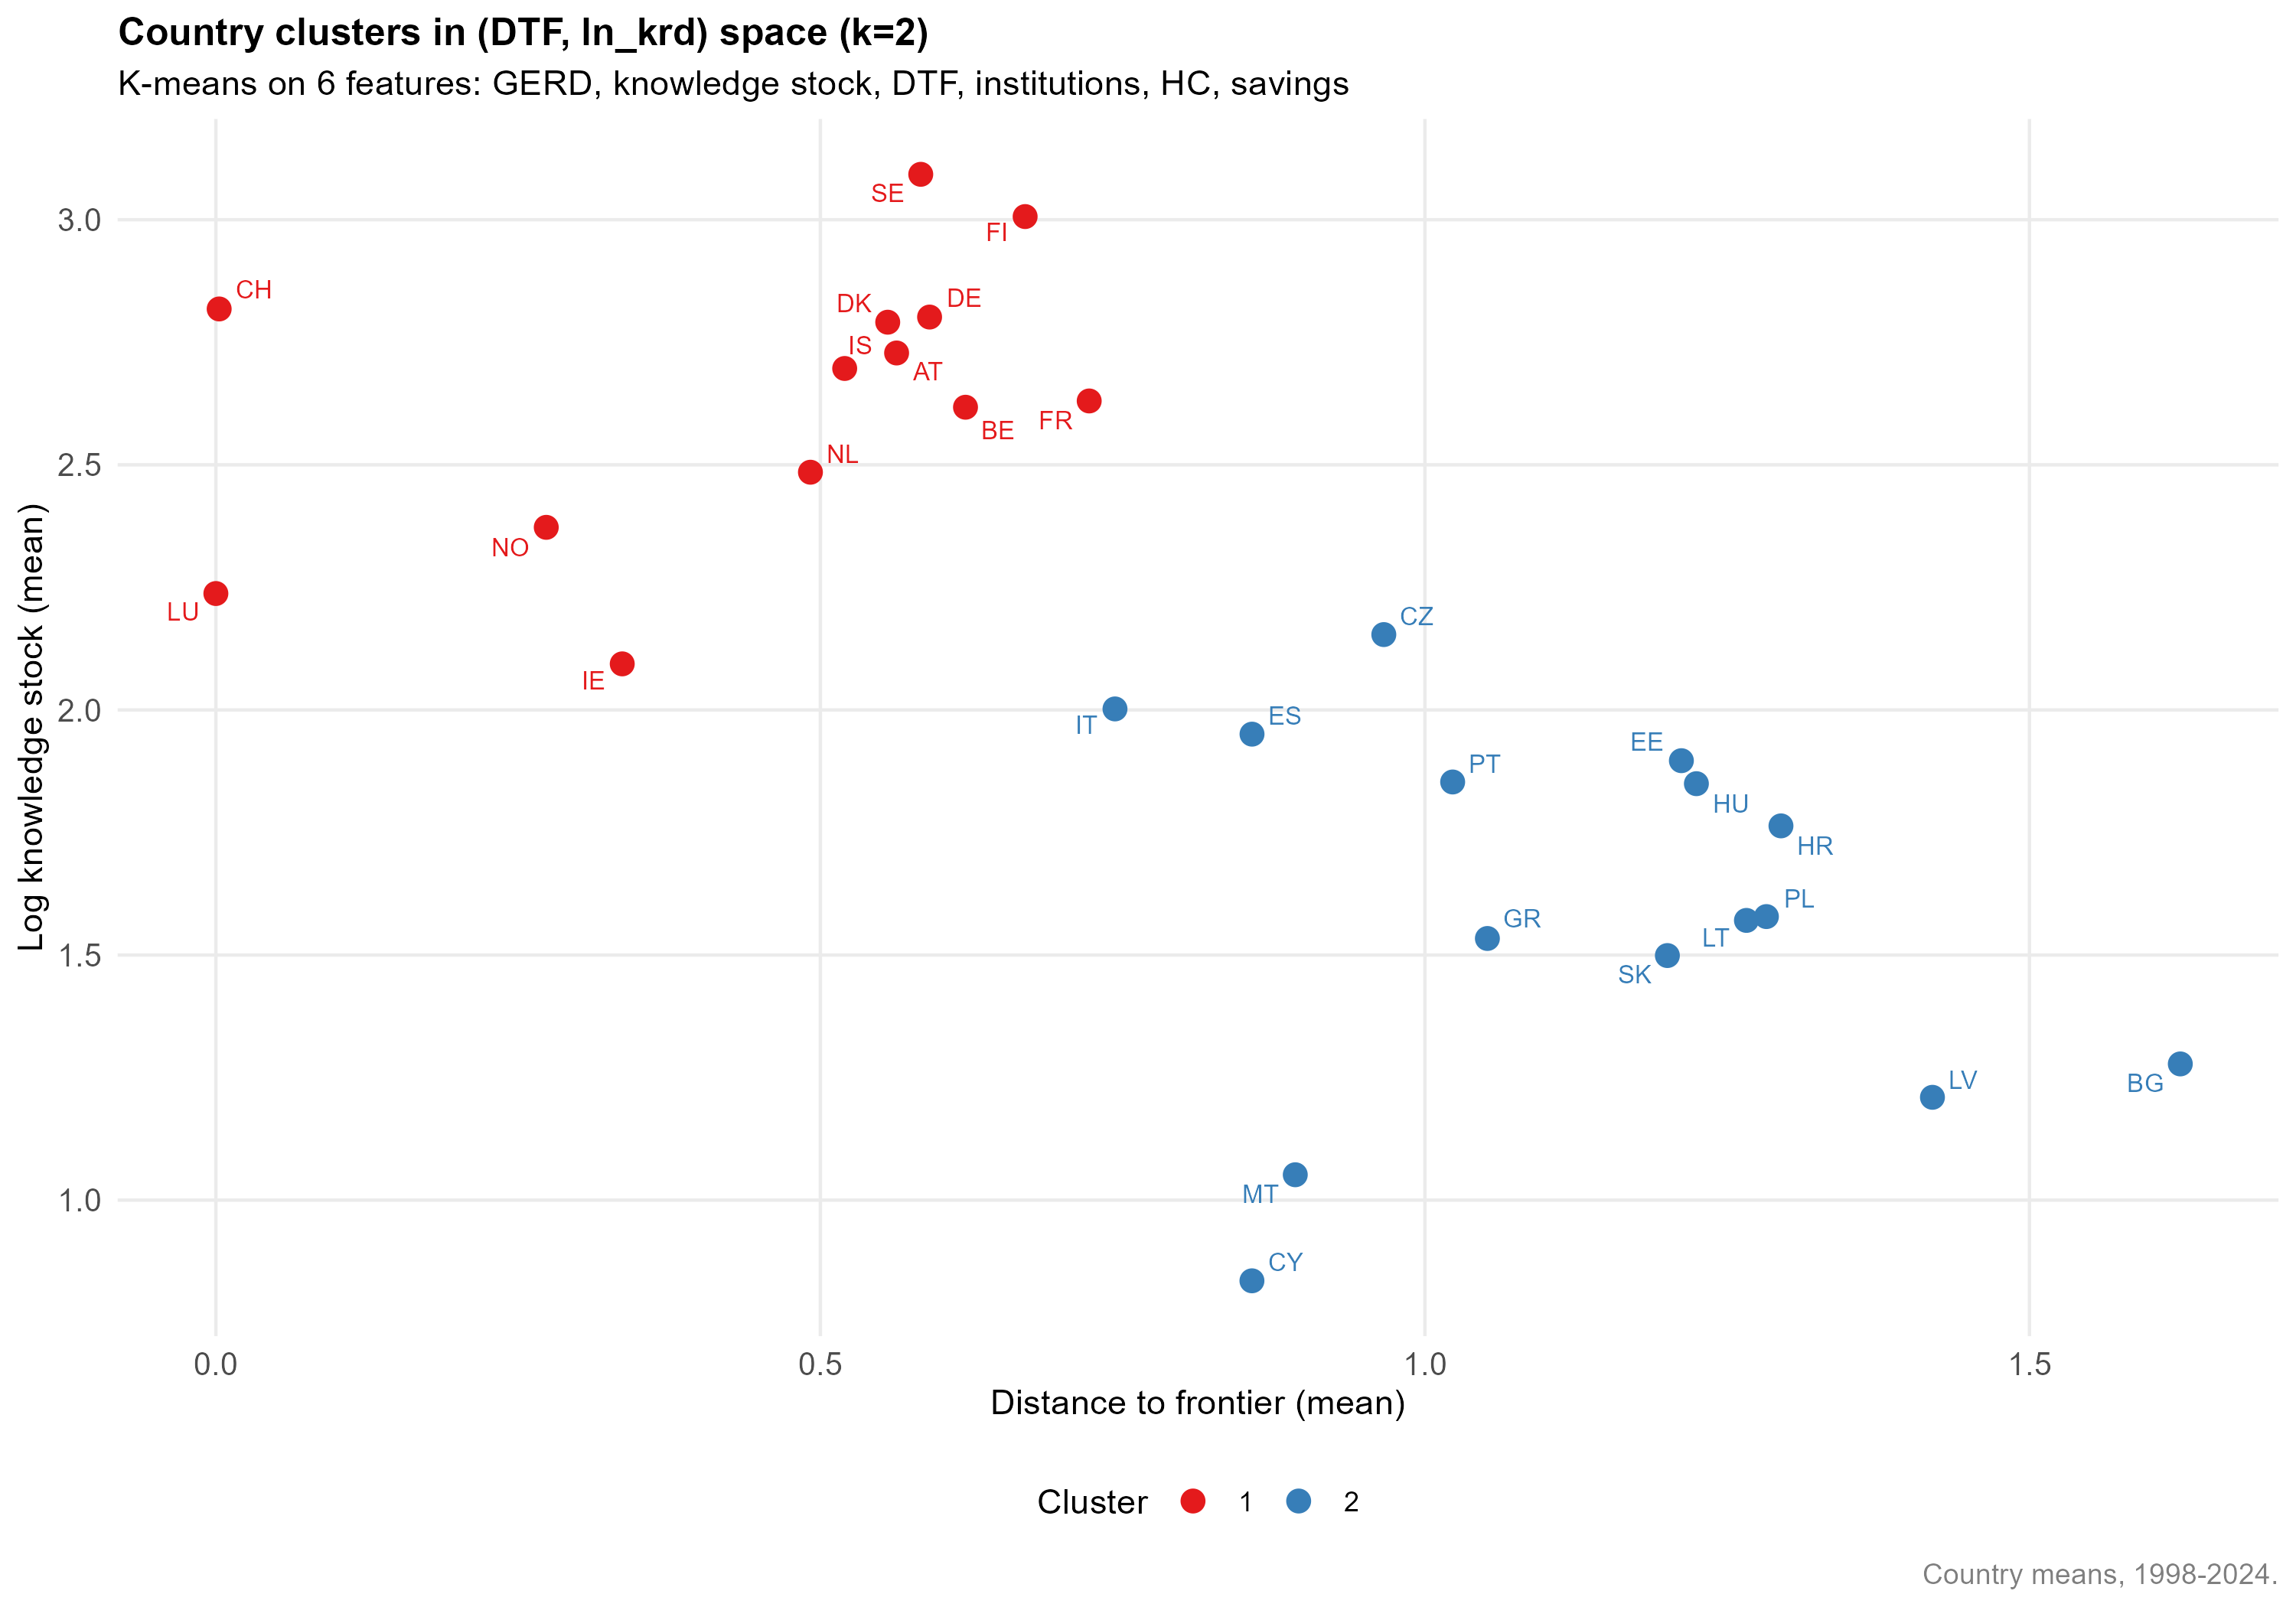
\includegraphics[width=0.95\linewidth]{figures/08_scatter_dtf_krd} 

}

\caption{Country clusters in (DTF, ln knowledge stock) space. K-means with six features.}(\#fig:fig-scatter)
\end{figure}

\begin{figure}

{\centering 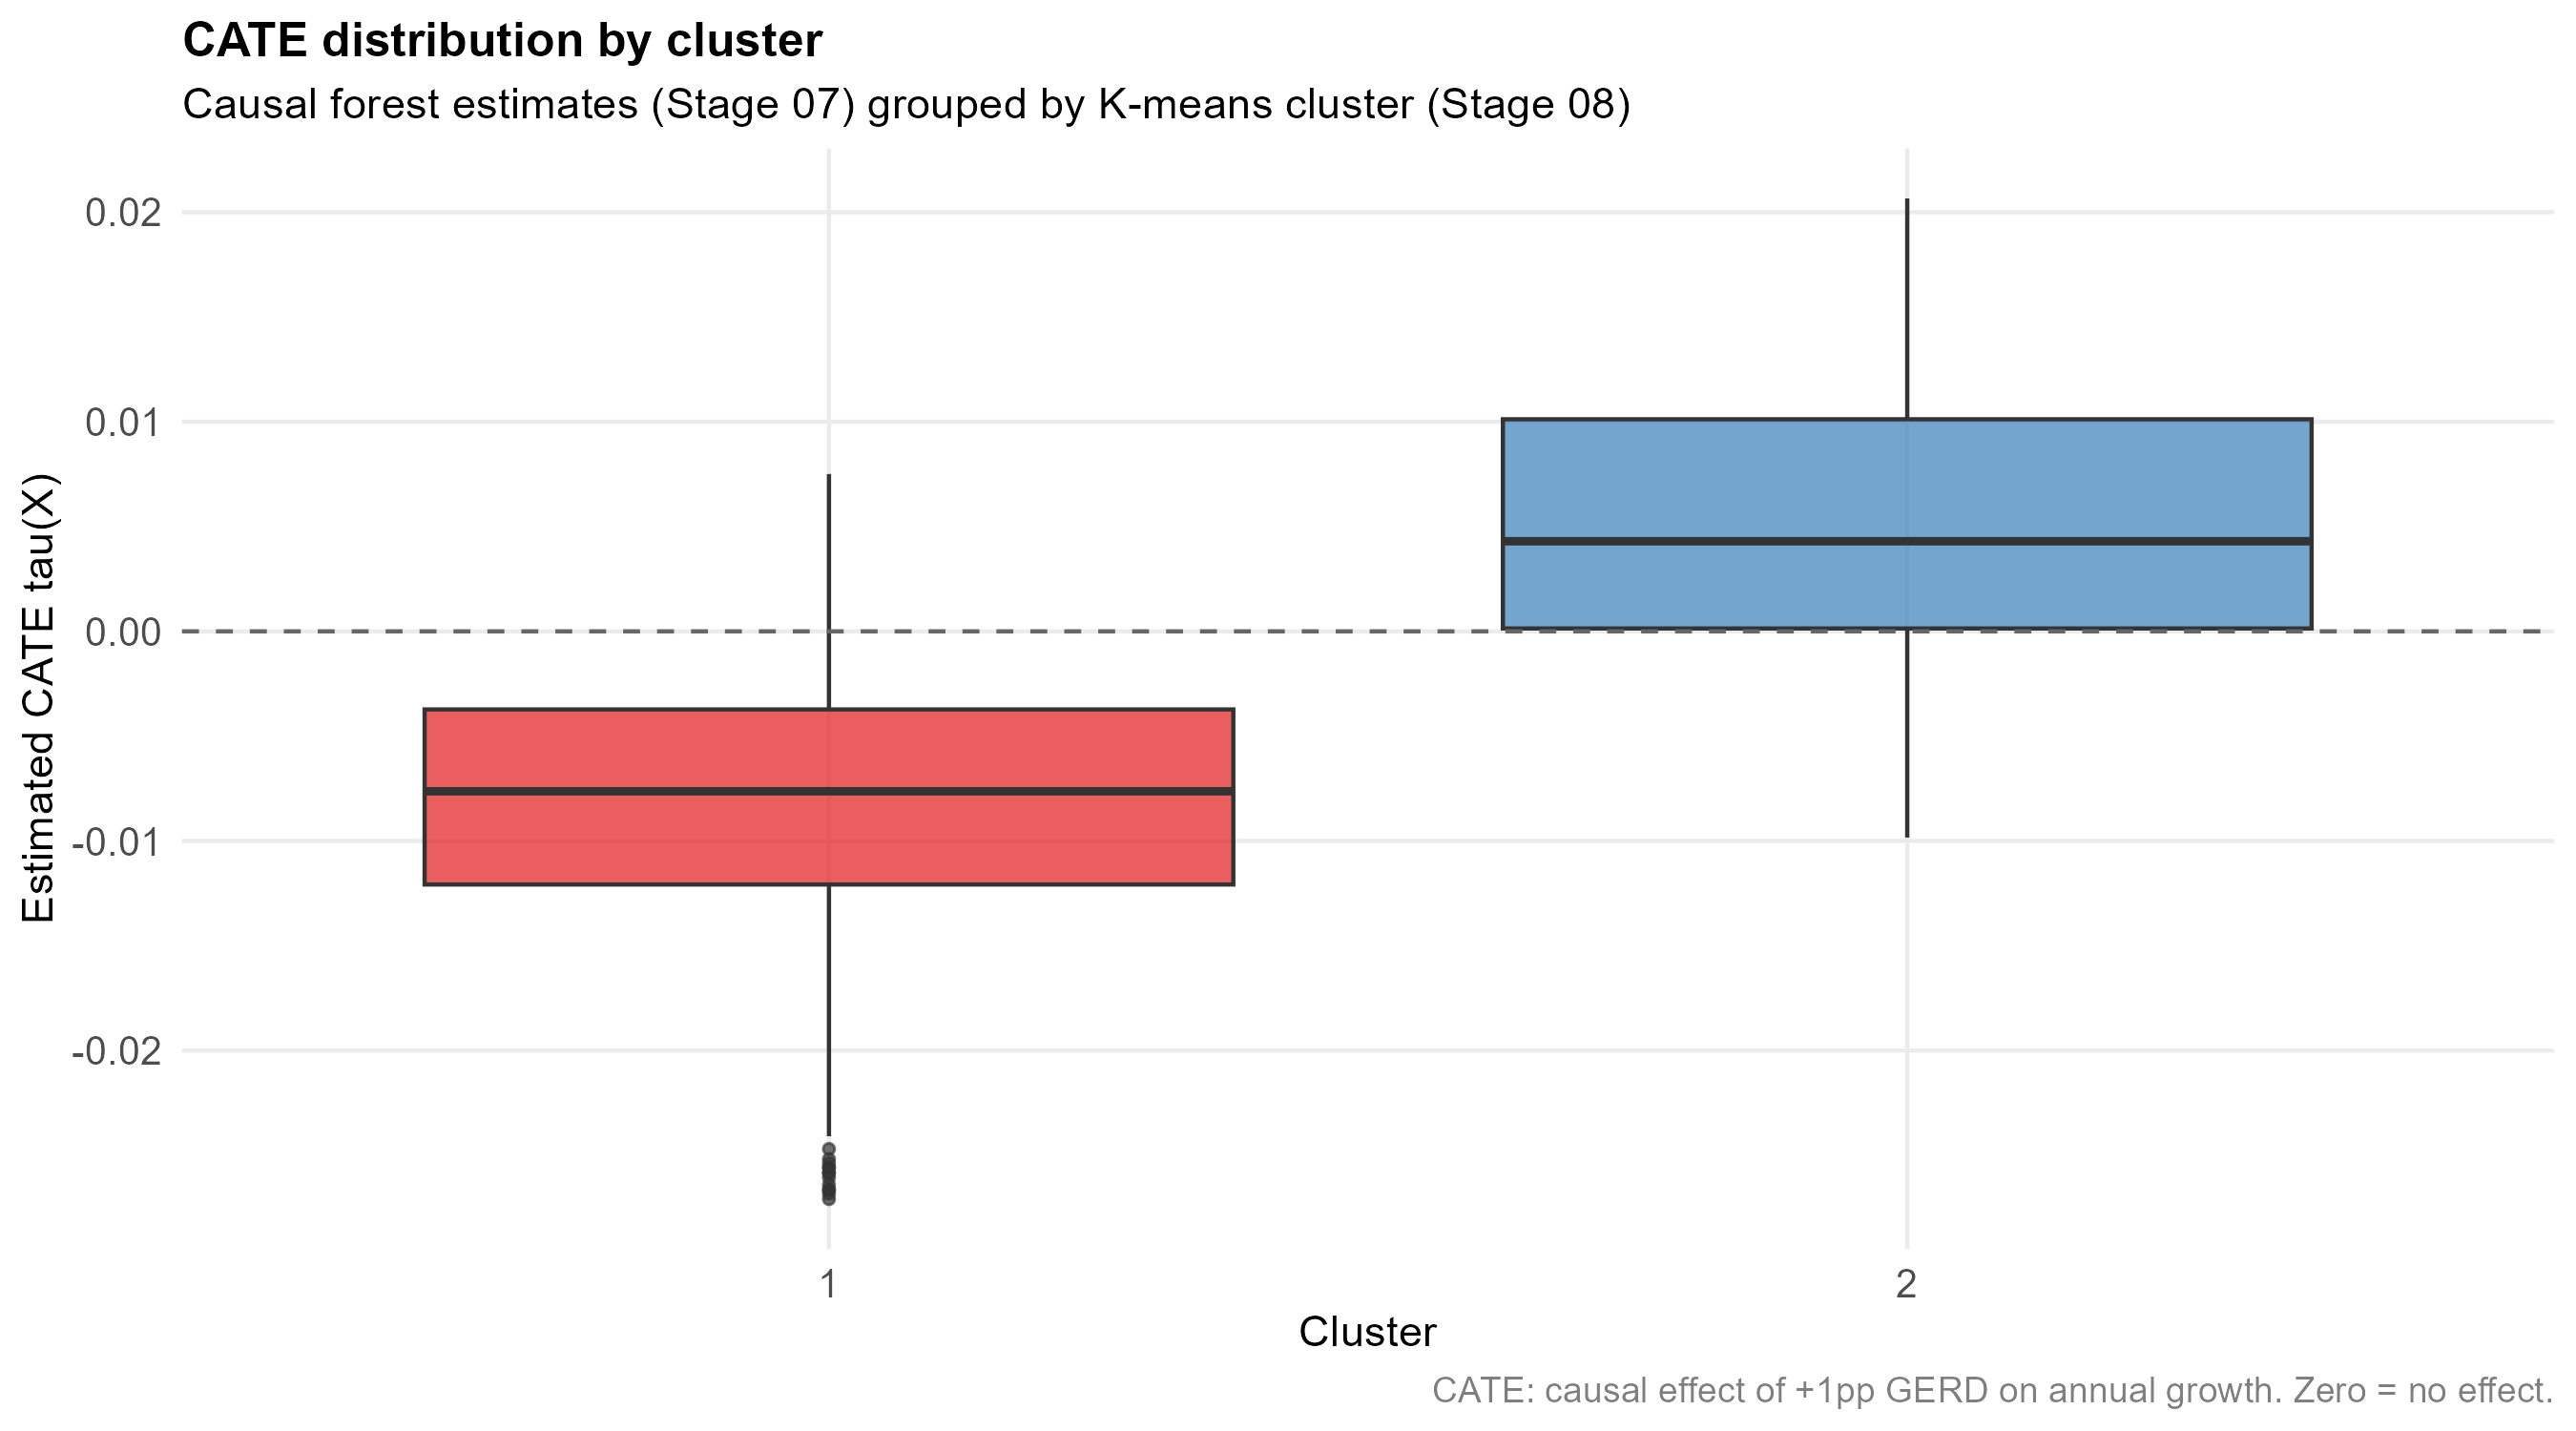
\includegraphics[width=0.95\linewidth]{figures/08_cate_by_cluster} 

}

\caption{CATE distribution by cluster. Causal forest estimates (Stage 07) grouped by K-means cluster (Stage 08).}(\#fig:fig-cluster-cate)
\end{figure}

\hypertarget{sec:discussion}{%
\section{Discussion}\label{sec:discussion}}

\hypertarget{why-does-the-aggregate-gerd-effect-appear-null}{%
\subsection{Why Does the Aggregate GERD Effect Appear Null?}\label{why-does-the-aggregate-gerd-effect-appear-null}}

Four non-mutually-exclusive explanations are consistent with the evidence:

\textbf{1. Measurement error attenuation.} The Wu--Hausman test and the IV \(>\) FE finding confirm that classical measurement error in GERD suppresses the OLS/FE coefficient toward zero. Survey-based GERD captures expenditure but not quality, timing, or appropriability of R\&D investments. The true causal coefficient may be positive but is attenuated below detectability at the aggregate annual frequency.

\textbf{2. Opposing regime effects.} The frontier split in LP and clustering reveals that the GERD coefficient is approximately \(-0.008\) for Innovation Leaders and \(+0.005\) for Convergence Economies. These nearly cancel in the pooled estimator. This is consistent with the Aghion--Akcigit--Howitt model where the marginal return to own-innovation is lower---and potentially displaced by spillouts---near the frontier (\protect\hyperlink{ref-aghion2014}{Aghion, Akcigit, and Howitt 2014}).

\textbf{3. Ideas becoming harder to find.} \protect\hyperlink{ref-bloom2020}{Bloom et al.} (\protect\hyperlink{ref-bloom2020}{2020}) document a secular decline in research productivity across multiple sectors. If each percentage-point of GERD generates a smaller TFP increment over time, any positive coefficient would weaken in a long panel. The research-productivity measure constructed in Stage 01 (Stage 03 feature engineering) shows declining trends consistent with this mechanism, though we do not test it formally here.

\textbf{4. Long lags and horizon mismatch.} The LP analysis shows that even where effects exist, they emerge primarily at \(h = 6\)--\(8\) years (catch-up economies) or are small and transient (frontier economies). Annual growth regressions with contemporaneous GERD are misaligned with this lag structure, contributing to the null finding at \(h = 0\).

\hypertarget{spatial-knowledge-flows-at-the-macro-level}{%
\subsection{Spatial Knowledge Flows at the Macro Level}\label{spatial-knowledge-flows-at-the-macro-level}}

The absence of statistically significant spatial spillovers (\(\lambda = 0.107\), \(p = 0.33\); \(W\text{GERD}\) coefficients non-significant across all three weight matrices) stands in contrast to the microeconomic evidence of \protect\hyperlink{ref-jaffe1986}{Jaffe} (\protect\hyperlink{ref-jaffe1986}{1986}) and the bilateral trade channel documented by \protect\hyperlink{ref-coe1995}{Coe and Helpman} (\protect\hyperlink{ref-coe1995}{1995}). Several explanations are possible. Two-way year fixed effects absorb common technology shocks (the main transmission channel in \protect\hyperlink{ref-coe1995}{Coe and Helpman} (\protect\hyperlink{ref-coe1995}{1995})), leaving only residual spatial correlation to identify. At the aggregate GERD-to-GDP-growth level, the channel from neighbours' R\&D spending to own country growth may operate through trade and FDI flows that are not spatially localised in the way capital-city distance suggests.

\hypertarget{policy-implications}{%
\subsection{Policy Implications}\label{policy-implications}}

The findings carry a cautious implication for R\&D policy in Europe. A uniform expansion of GERD spending---as targeted by the 3\% of GDP Barcelona objective---is unlikely to generate detectable aggregate growth gains at the annual frequency. The benefits, if any, accrue over long lags and are more plausibly realized through knowledge absorption in convergence economies than through innovation in frontier economies. Human capital (tertiary attainment, absorptive capacity interaction) and institutional quality emerge as complementary conditions with CATE-relevance, suggesting that R\&D subsidies bundled with education investment and governance improvements may be more effective than standalone spending mandates.

\hypertarget{sec:conclusion}{%
\section{Conclusion}\label{sec:conclusion}}

This paper has assembled a comprehensive empirical case study of the GERD--growth relationship in European economies. The central finding is that, once cross-sectional dependence is properly accounted for with Driscoll--Kraay standard errors, the aggregate association between R\&D spending and annual GDP-per-capita growth is statistically indistinguishable from zero. This finding is robust across two-way fixed effects, Anderson--Hsiao IV, local projections at all horizons \(h \leq 7\) for the full panel, three spatial weight matrices, double/debiased ML with ridge nuisance, and causal forests.

The null does not, however, imply that R\&D is irrelevant. The frontier-split local projections reveal persistent negative direct effects for close-to-frontier economies and a delayed positive response for catch-up economies---a pattern theoretically coherent with the distance-to-frontier mechanism of \protect\hyperlink{ref-aghion2014}{Aghion, Akcigit, and Howitt} (\protect\hyperlink{ref-aghion2014}{2014}). The causal forest CATE estimates corroborate this: Innovation Leaders (Cluster 1) exhibit mean CATE \(\approx -0.008\) while Convergence Economies (Cluster 2) show mean CATE \(\approx +0.005\), generating the near-zero aggregate average. Measurement error attenuation (IV \(>\) FE, Wu--Hausman \(p = 0.004\)) implies the true coefficient is likely positive but small, attenuated below detectability by survey noise in GERD.

Factor accumulation---savings rates and population growth plus depreciation---remains the dominant, consistently significant channel across all six analytical stages, consistent with the augmented Solow model of \protect\hyperlink{ref-mankiw1992}{Mankiw, Romer, and Weil} (\protect\hyperlink{ref-mankiw1992}{1992}). Europe's near-term growth performance appears more tightly tied to capital deepening and demographic dynamics than to R\&D intensity at the aggregate annual scale.

Future work could extend this analysis in three directions. First, disaggregating GERD by sector (business, government, higher education) and funding source (public, private) would allow sharper identification of the mechanism. Second, firm-level matched panel data would eliminate measurement error at the country level and allow estimation of micro-level returns. Third, extending the spatial model to include explicit bilateral trade and FDI weights---rather than geographic distance---would provide a more direct test of the Coe--Helpman knowledge-diffusion channel.

\hypertarget{references}{%
\section*{References}\label{references}}
\addcontentsline{toc}{section}{References}

\hypertarget{refs}{}
\begin{CSLReferences}{1}{0}
\leavevmode\vadjust pre{\hypertarget{ref-aghion2014}{}}%
Aghion, Philippe, Ufuk Akcigit, and Peter Howitt. 2014. {``What Do We Learn from {Schumpeterian} Growth Theory?''} Edited by Philippe Aghion and Steven N. Durlauf 2: 515--63. \url{https://doi.org/10.1016/B978-0-444-53540-5.00001-X}.

\leavevmode\vadjust pre{\hypertarget{ref-aghion1992}{}}%
Aghion, Philippe, and Peter Howitt. 1992. {``A Model of Growth Through Creative Destruction.''} \emph{Econometrica} 60 (2): 323--51. \url{https://doi.org/10.2307/2951599}.

\leavevmode\vadjust pre{\hypertarget{ref-fixest2023}{}}%
Bergé, Laurent. 2023. \emph{{fixest}: Fast Fixed-Effects Estimations}. \url{https://CRAN.R-project.org/package=fixest}.

\leavevmode\vadjust pre{\hypertarget{ref-bloom2020}{}}%
Bloom, Nicholas, Charles I. Jones, John Van Reenen, and Michael Webb. 2020. {``Are Ideas Getting Harder to Find?''} \emph{American Economic Review} 110 (4): 1104--44. \url{https://doi.org/10.1257/aer.20180338}.

\leavevmode\vadjust pre{\hypertarget{ref-chernozhukov2018}{}}%
Chernozhukov, Victor, Denis Chetverikov, Mert Demirer, Esther Duflo, Christian Hansen, Whitney Newey, and James Robins. 2018. {``Double/Debiased Machine Learning for Treatment and Structural Parameters.''} \emph{Econometrics Journal} 21 (1): C1--68. \url{https://doi.org/10.1111/ectj.12097}.

\leavevmode\vadjust pre{\hypertarget{ref-coe1995}{}}%
Coe, David T., and Elhanan Helpman. 1995. {``International {R\&D} Spillovers.''} \emph{European Economic Review} 39 (5): 859--87. \url{https://doi.org/10.1016/0014-2921(94)00100-E}.

\leavevmode\vadjust pre{\hypertarget{ref-driscollkraay1998}{}}%
Driscoll, John C., and Aart C. Kraay. 1998. {``Consistent Covariance Matrix Estimation with Spatially Dependent Panel Data.''} \emph{Review of Economics and Statistics} 80 (4): 549--60. \url{https://doi.org/10.1162/003465398557825}.

\leavevmode\vadjust pre{\hypertarget{ref-eurostat_gdp}{}}%
Eurostat. 2024. \emph{{GDP} and Main Components: Output, Expenditure and Income {[}{nama\_10\_pc}{]}}. \url{https://ec.europa.eu/eurostat/data/database}.

\leavevmode\vadjust pre{\hypertarget{ref-pwt100}{}}%
Feenstra, Robert C., Robert Inklaar, and Marcel P. Timmer. 2021. \emph{Penn World Table, Version 10.0}. \url{https://doi.org/10.15141/S5J01T}.

\leavevmode\vadjust pre{\hypertarget{ref-griliches1979}{}}%
Griliches, Zvi. 1979. {``Issues in Assessing the Contribution of Research and Development to Productivity Growth.''} \emph{Bell Journal of Economics} 10 (1): 92--116. \url{https://doi.org/10.2307/3003321}.

\leavevmode\vadjust pre{\hypertarget{ref-hall2010}{}}%
Hall, Bronwyn H., Jacques Mairesse, and Pierre Mohnen. 2010. {``Measuring the Returns to {R\&D}.''} Edited by Bronwyn H. Hall and Nathan Rosenberg 2: 1033--82. \url{https://doi.org/10.1016/S0169-7218(10)02008-3}.

\leavevmode\vadjust pre{\hypertarget{ref-hauk2009}{}}%
Hauk, William R., and Romain Wacziarg. 2009. {``A Monte Carlo Study of Growth Regressions.''} \emph{Journal of Economic Growth} 14 (2): 103--47. \url{https://doi.org/10.1007/s10887-009-9040-3}.

\leavevmode\vadjust pre{\hypertarget{ref-hausman1978}{}}%
Hausman, Jerry A. 1978. {``Specification Tests in Econometrics.''} \emph{Econometrica} 46 (6): 1251--71. \url{https://doi.org/10.2307/1913827}.

\leavevmode\vadjust pre{\hypertarget{ref-jaffe1986}{}}%
Jaffe, Adam B. 1986. {``Technological Opportunity and Spillovers of {R\&D}: Evidence from Firms' Patents, Profits, and Market Value.''} \emph{American Economic Review} 76 (5): 984--1001.

\leavevmode\vadjust pre{\hypertarget{ref-jorda2005}{}}%
Jordà, Òscar. 2005. {``Estimation and Inference of Impulse Responses by Local Projections.''} \emph{American Economic Review} 95 (1): 161--82. \url{https://doi.org/10.1257/0002828053828518}.

\leavevmode\vadjust pre{\hypertarget{ref-knaus2021}{}}%
Knaus, Michael C., Michael Lechner, and Anthony Strittmatter. 2021. {``Machine Learning Estimation of Heterogeneous Causal Effects: Empirical Monte Carlo Evidence.''} \emph{Econometrics Journal} 24 (1): 134--61. \url{https://doi.org/10.1093/ectj/utaa014}.

\leavevmode\vadjust pre{\hypertarget{ref-lesagepace2009}{}}%
LeSage, James, and R. Kelley Pace. 2009. \emph{Introduction to Spatial Econometrics}. Chapman; Hall/CRC. \url{https://doi.org/10.1201/9781420064254}.

\leavevmode\vadjust pre{\hypertarget{ref-mankiw1992}{}}%
Mankiw, N. Gregory, David Romer, and David N. Weil. 1992. {``A Contribution to the Empirics of Economic Growth.''} \emph{Quarterly Journal of Economics} 107 (2): 407--37. \url{https://doi.org/10.2307/2118477}.

\leavevmode\vadjust pre{\hypertarget{ref-nelsonphelps1966}{}}%
Nelson, Richard R., and Edmund S. Phelps. 1966. {``Investment in Humans, Technological Diffusion, and Economic Growth.''} \emph{American Economic Review} 56 (1/2): 69--75.

\leavevmode\vadjust pre{\hypertarget{ref-oecd_msti}{}}%
OECD. 2024. \emph{Main Science and Technology Indicators ({MSTI})}. \url{https://www.oecd.org/sti/msti.htm}.

\leavevmode\vadjust pre{\hypertarget{ref-pesaran2021}{}}%
Pesaran, M. Hashem. 2021. {``General Diagnostic Tests for Cross-Sectional Dependence in Panels.''} \emph{Empirical Economics} 60: 13--50. \url{https://doi.org/10.1007/s00181-020-01875-7}.

\leavevmode\vadjust pre{\hypertarget{ref-ramey2018}{}}%
Ramey, Valerie A., and Sarah Zubairy. 2018. {``Government Spending Multipliers in Good Times and in Bad: Evidence from {US} Historical Data.''} \emph{Journal of Political Economy} 126 (2): 850--901. \url{https://doi.org/10.1086/696277}.

\leavevmode\vadjust pre{\hypertarget{ref-roodman2009}{}}%
Roodman, David. 2009. {``A Note on the Theme of Too Many Instruments.''} \emph{Oxford Bulletin of Economics and Statistics} 71 (1): 135--58. \url{https://doi.org/10.1111/j.1468-0084.2008.00542.x}.

\leavevmode\vadjust pre{\hypertarget{ref-wagerathey2018}{}}%
Wager, Stefan, and Susan Athey. 2018. {``Estimation and Inference of Heterogeneous Treatment Effects Using Random Forests.''} \emph{Journal of the American Statistical Association} 113 (523): 1228--42. \url{https://doi.org/10.1080/01621459.2017.1319839}.

\leavevmode\vadjust pre{\hypertarget{ref-worldbank_wgi}{}}%
World Bank. 2024. \emph{Worldwide Governance Indicators ({WGI})}. \url{https://www.worldbank.org/en/publication/worldwide-governance-indicators}.

\end{CSLReferences}

\newpage

\hypertarget{appendix}{%
\section*{Appendix}\label{appendix}}
\addcontentsline{toc}{section}{Appendix}

\hypertarget{data-coverage}{%
\subsection*{Data Coverage}\label{data-coverage}}
\addcontentsline{toc}{subsection}{Data Coverage}

\begin{figure}

{\centering 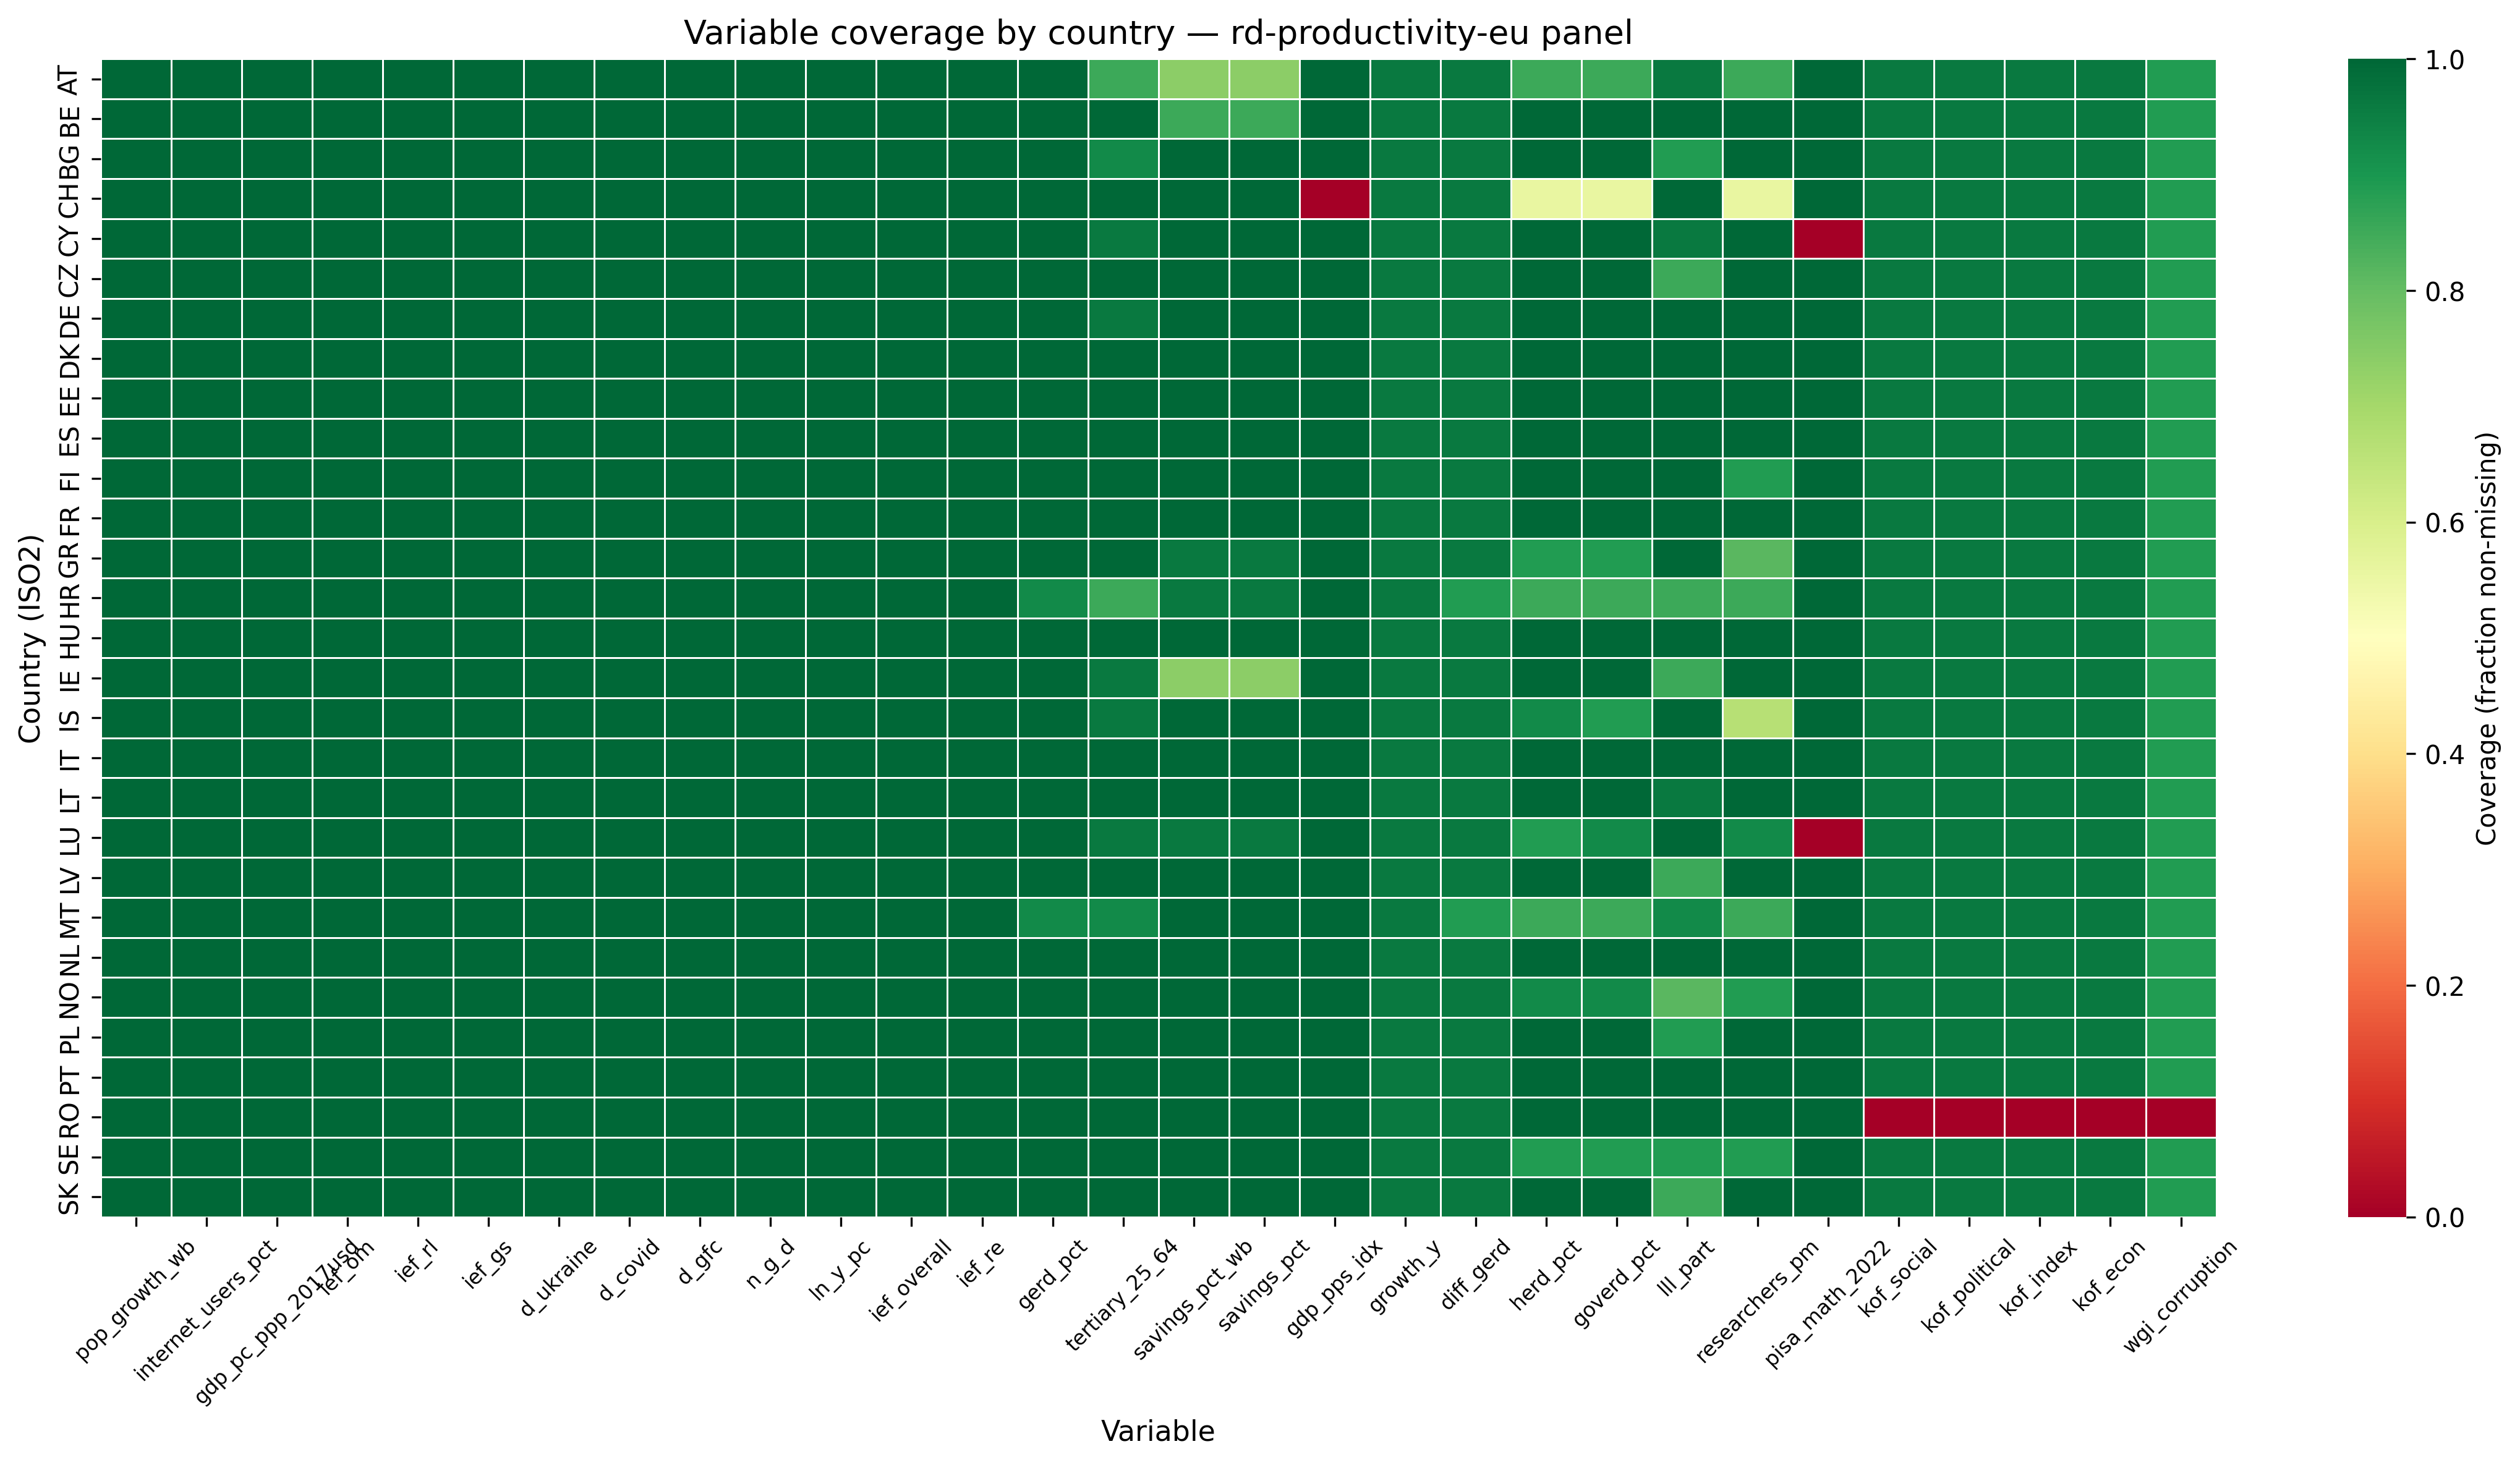
\includegraphics[width=0.95\linewidth]{figures/01_coverage_heatmap} 

}

\caption{Data coverage heatmap: non-missing observations by country and variable.}(\#fig:fig-coverage)
\end{figure}

\hypertarget{panel-spaghetti-plot}{%
\subsection*{Panel Spaghetti Plot}\label{panel-spaghetti-plot}}
\addcontentsline{toc}{subsection}{Panel Spaghetti Plot}

\begin{figure}

{\centering 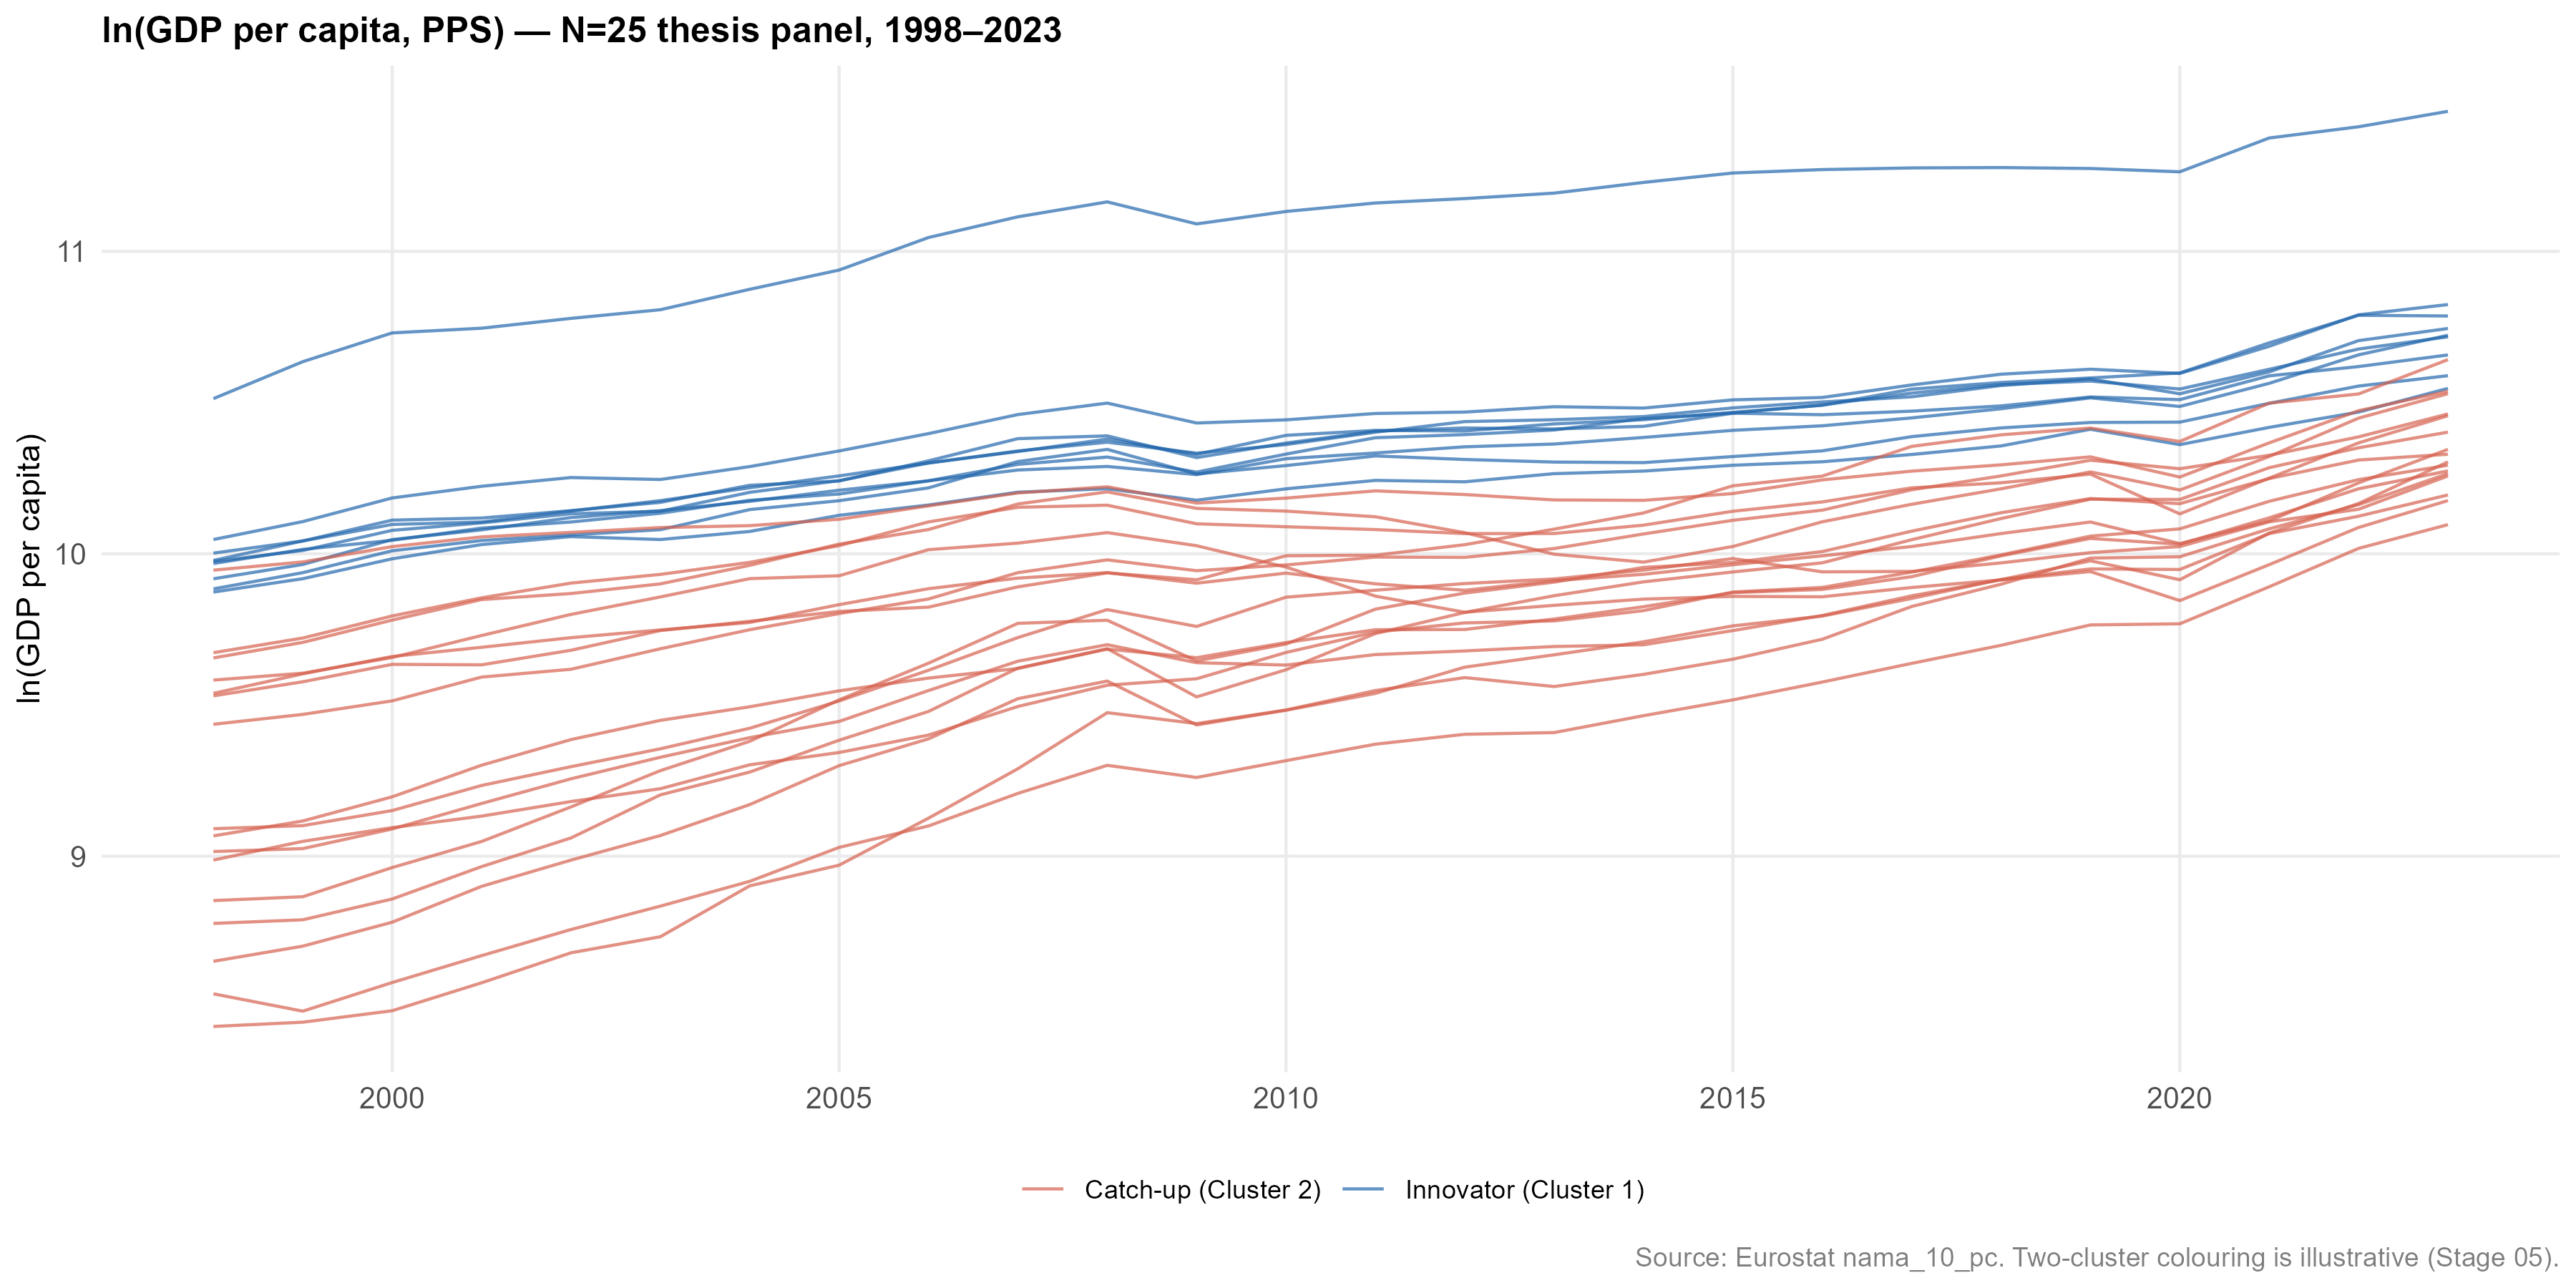
\includegraphics[width=0.95\linewidth]{figures/02_panel_spaghetti} 

}

\caption{Log GDP per capita trajectories, 1998--2024. Highlighted: N=29 primary panel.}(\#fig:fig-spaghetti)
\end{figure}

\hypertarget{dtfgrowth-scatter}{%
\subsection*{DTF--Growth Scatter}\label{dtfgrowth-scatter}}
\addcontentsline{toc}{subsection}{DTF--Growth Scatter}

\begin{figure}

{\centering 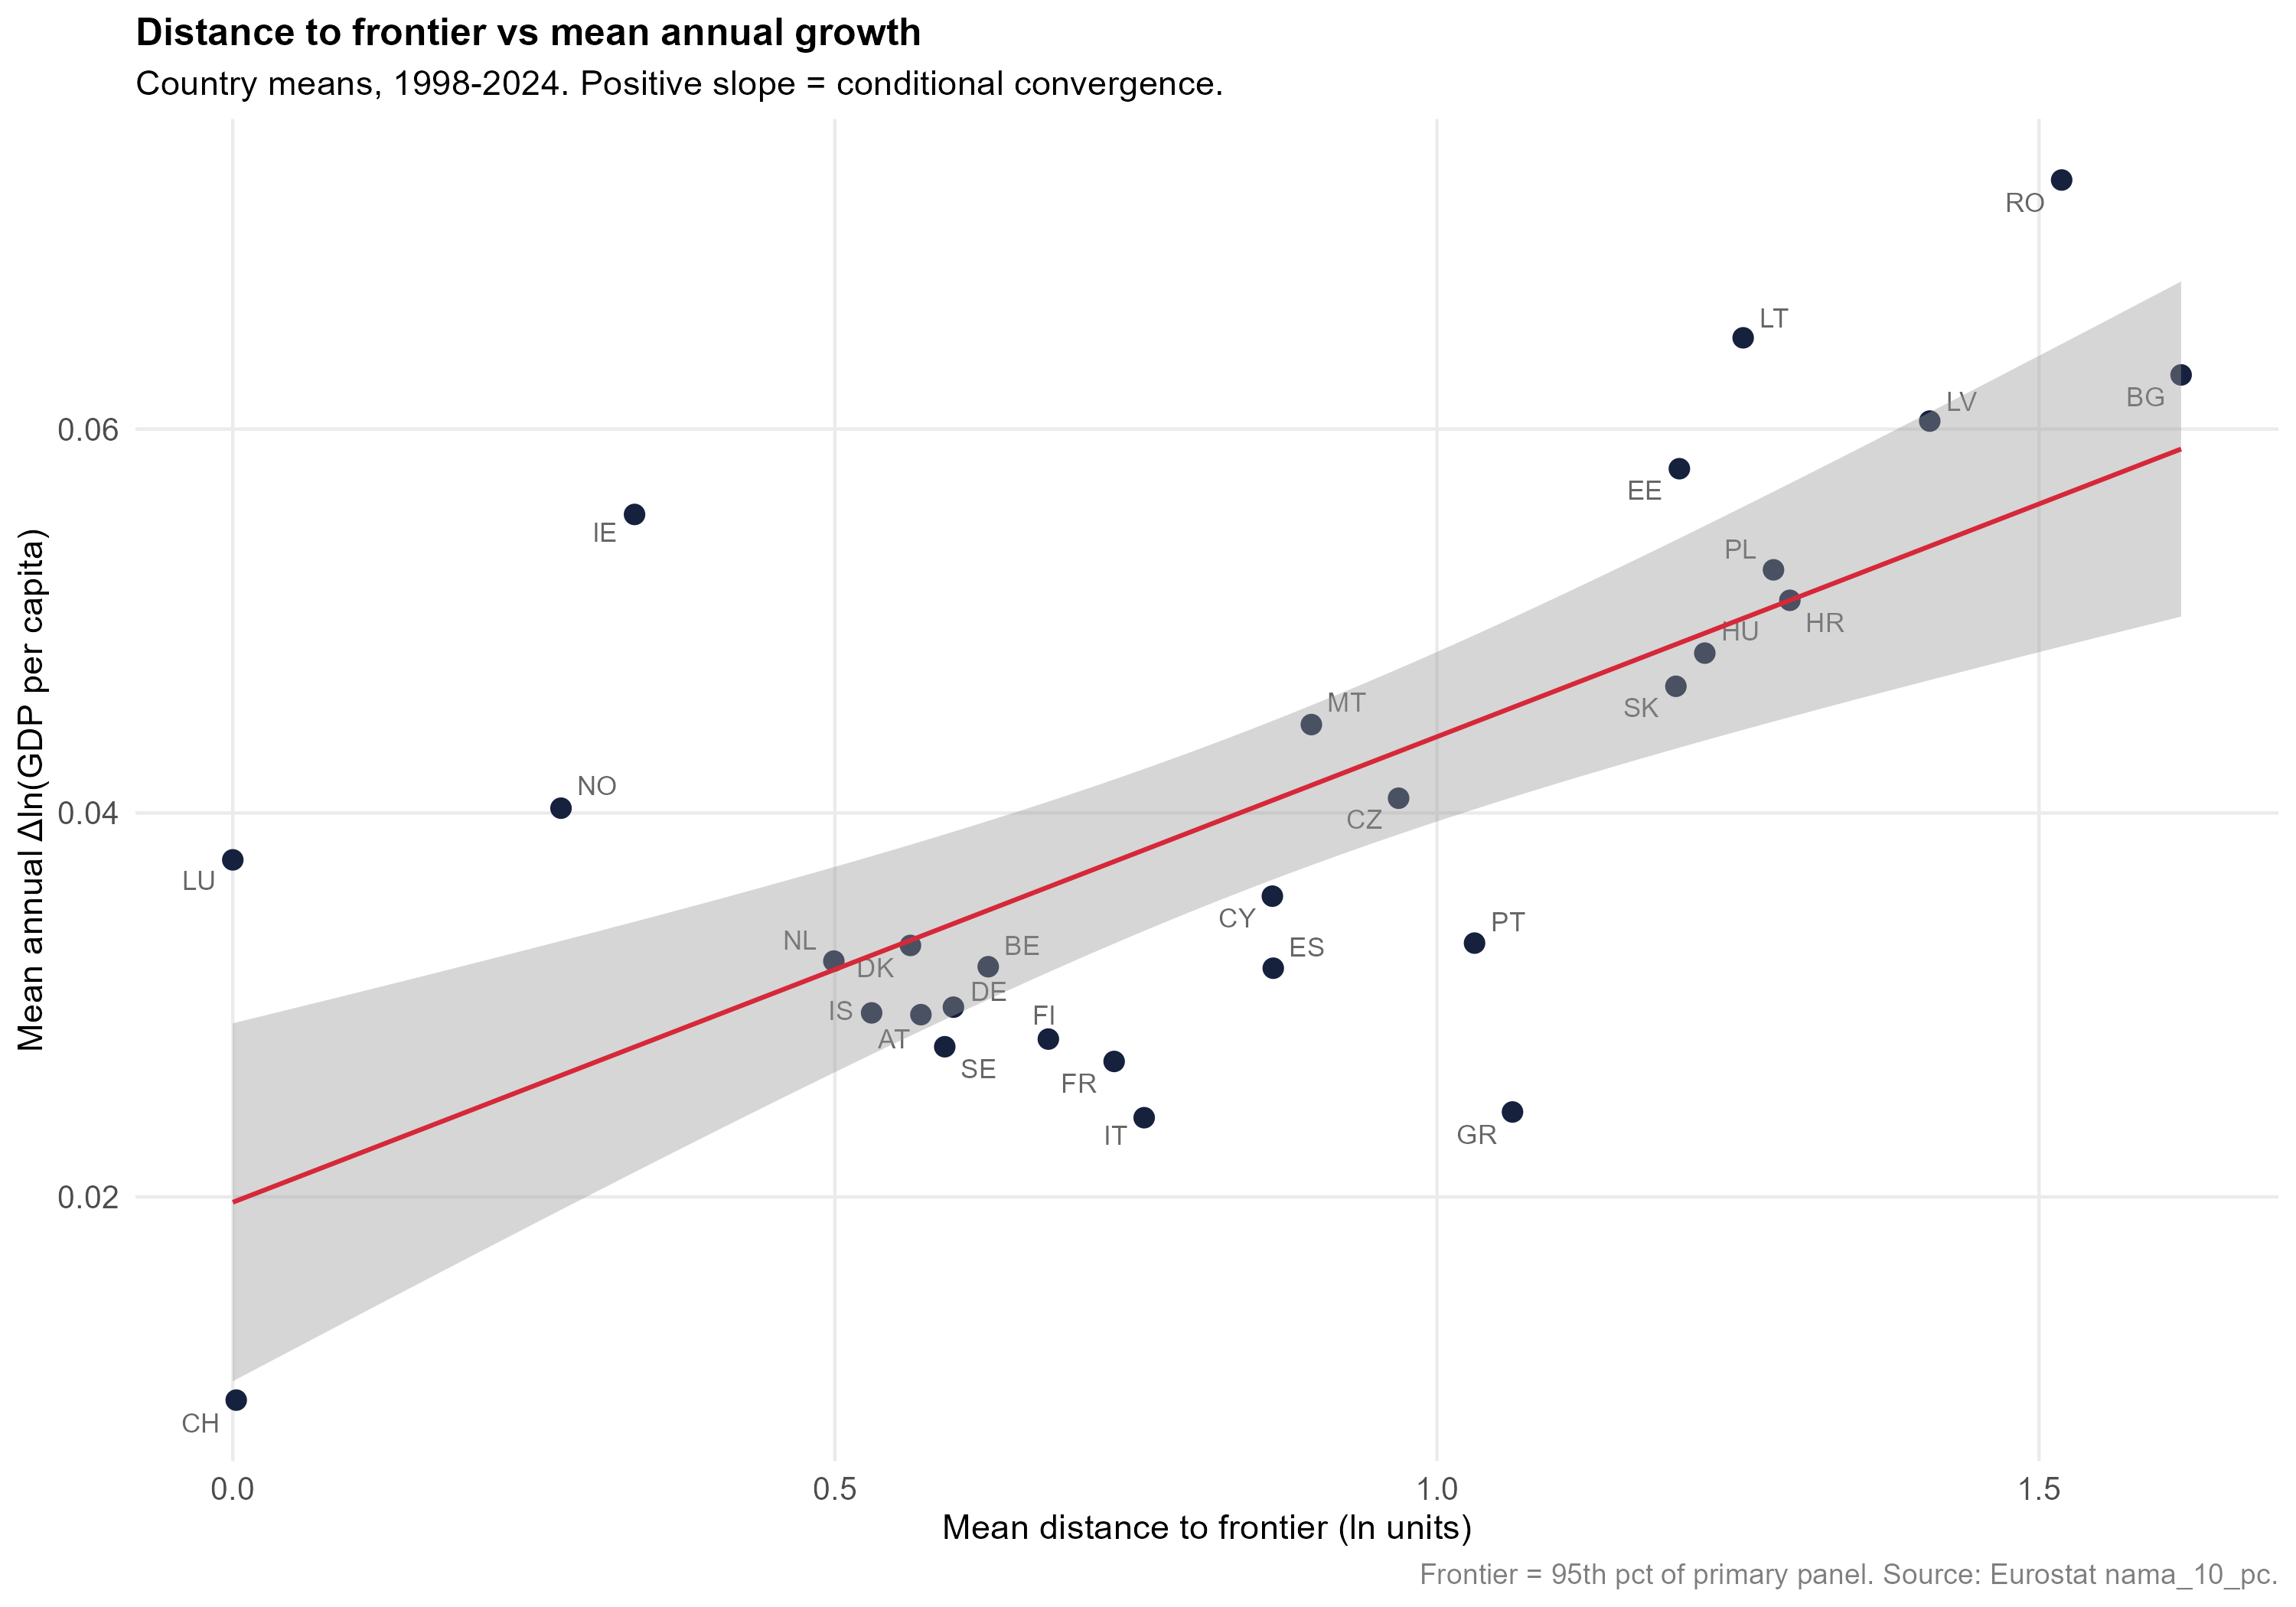
\includegraphics[width=0.95\linewidth]{figures/03_dtf_scatter} 

}

\caption{Country-mean distance to frontier vs mean annual growth. Positive slope indicates conditional convergence.}(\#fig:fig-dtf)
\end{figure}

\hypertarget{k-means-diagnostics}{%
\subsection*{K-means Diagnostics}\label{k-means-diagnostics}}
\addcontentsline{toc}{subsection}{K-means Diagnostics}

\begin{table}[!h]
\centering
\caption{(\#tab:kmeans-diag-table)K-means diagnostics: total WCSS and average silhouette by k.}
\centering
\begin{tabular}[t]{rrr}
\toprule
k & Total WCSS & Avg. silhouette\\
\midrule
2 & 63.795 & 0.486\\
3 & 52.771 & 0.346\\
4 & 42.220 & 0.294\\
5 & 35.600 & 0.254\\
6 & 30.369 & 0.263\\
\bottomrule
\end{tabular}
\end{table}

\begin{figure}

{\centering 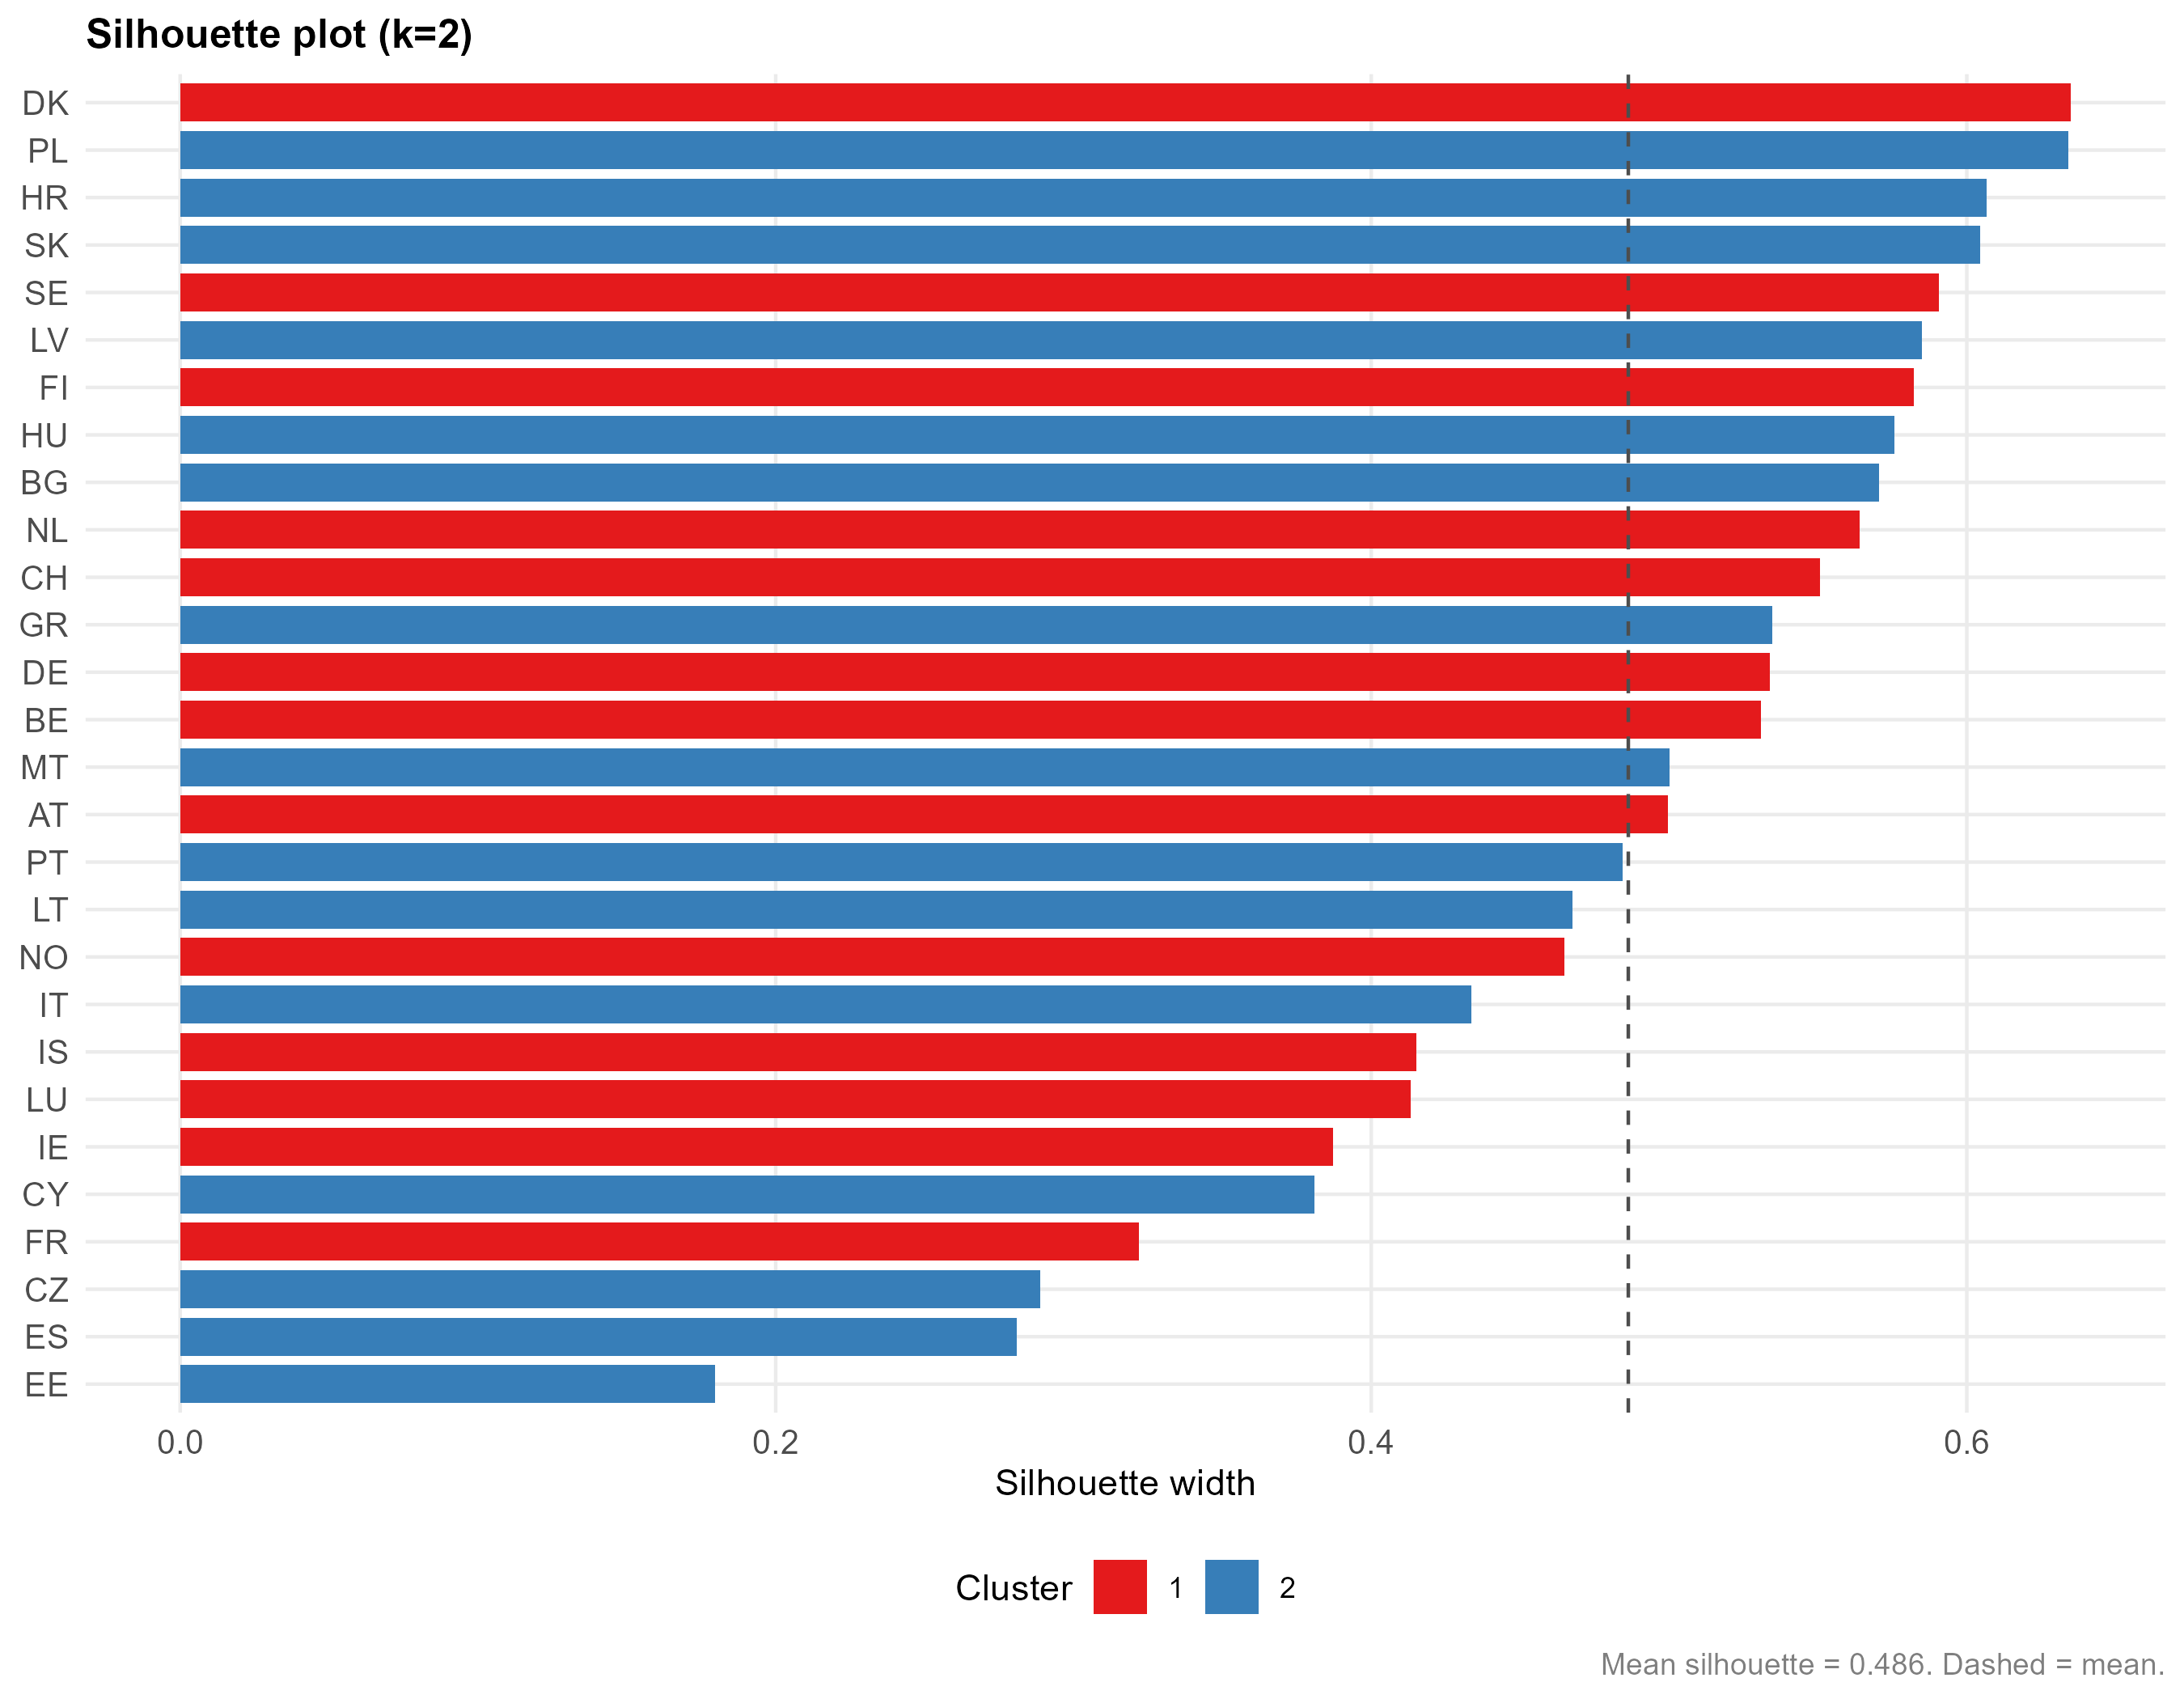
\includegraphics[width=0.95\linewidth]{figures/08_silhouette_obs} 

}

\caption{Silhouette plot (k=2): per-country silhouette widths.}(\#fig:fig-sil)
\end{figure}

\hypertarget{country-cate-estimates}{%
\subsection*{Country CATE Estimates}\label{country-cate-estimates}}
\addcontentsline{toc}{subsection}{Country CATE Estimates}

\begin{figure}

{\centering 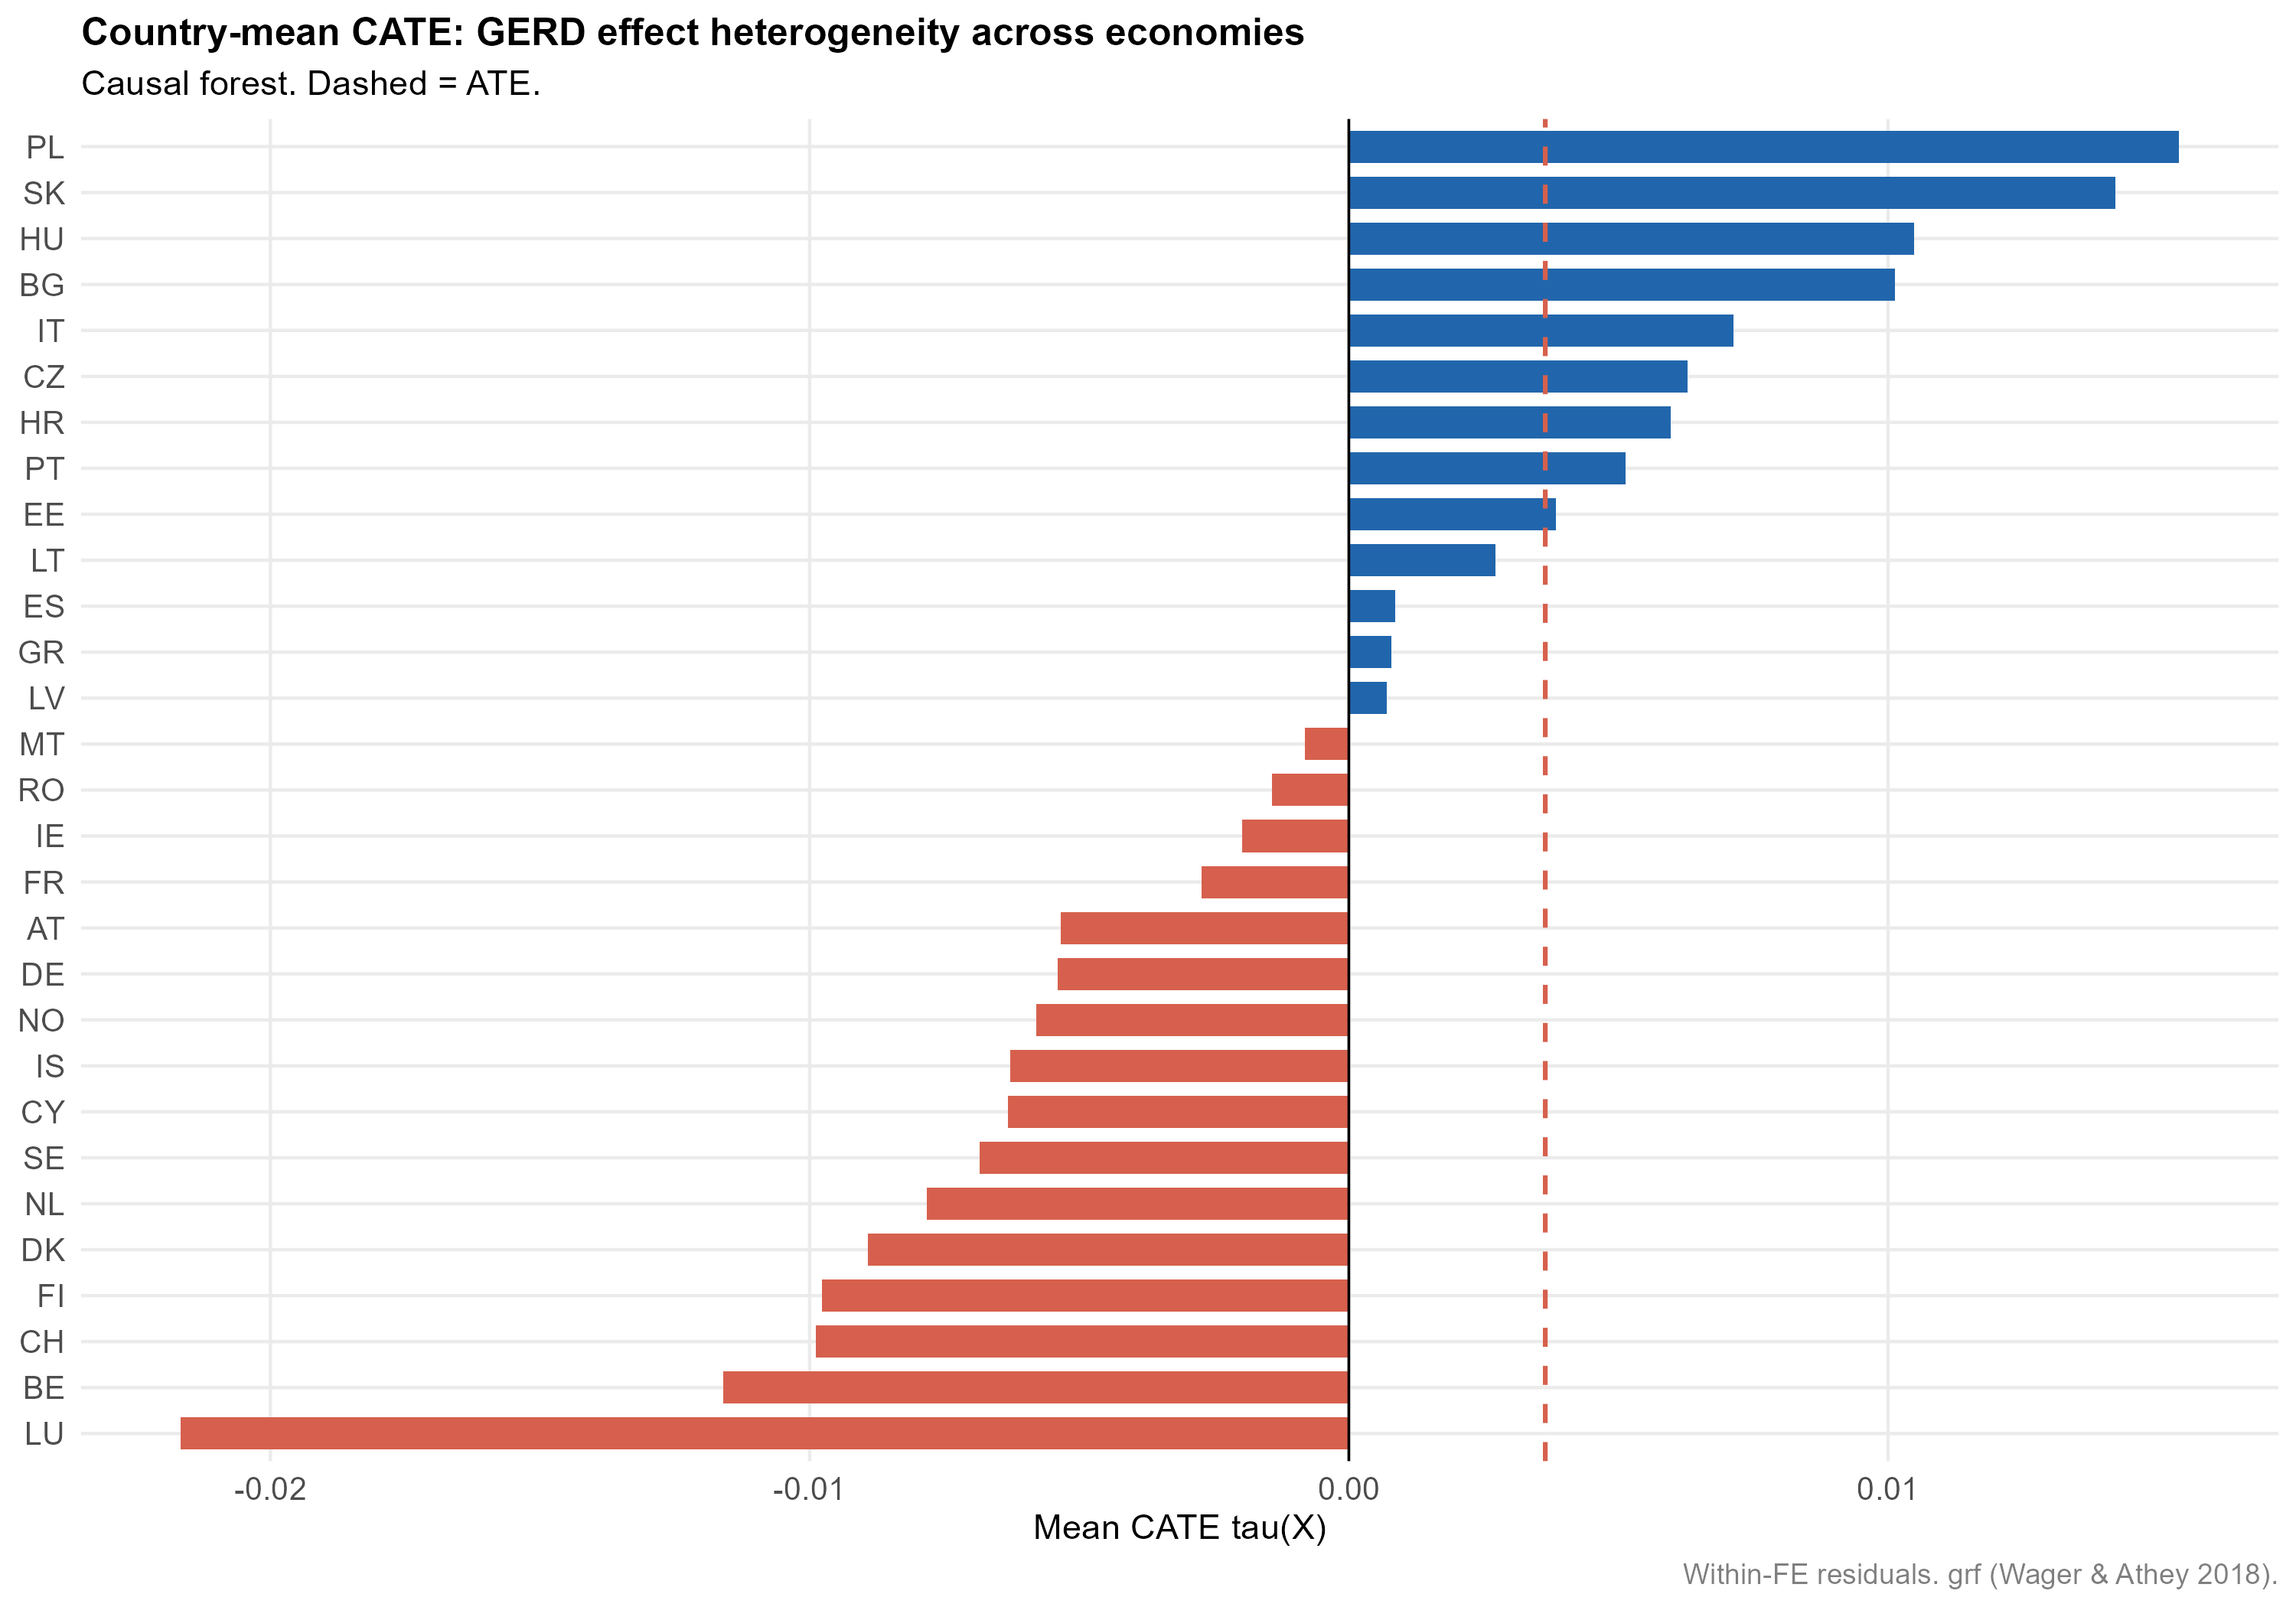
\includegraphics[width=0.95\linewidth]{figures/07_country_cate} 

}

\caption{Country-mean CATE estimates. Blue = positive effect, red = negative.}(\#fig:fig-country-cate)
\end{figure}

\end{document}
